% Risks (MDPI) manuscript draft for the stock index volatility project.
\documentclass[risks,article,submit,moreauthors]{Definitions/mdpi}

\usepackage{bm}   % bold math symbols (\bm) -- required for spillover feature notation

\setlength{\headheight}{24pt}

\firstpage{1}
\makeatletter
\setcounter{page}{\@firstpage}
\makeatother
\pubvolume{1}
\issuenum{1}
\articlenumber{0}
\pubyear{2026}
\copyrightyear{2026}
\datereceived{}
\daterevised{}
\dateaccepted{}
\datepublished{}
\Title{Public-Data Causal Multiscale Wavelet Spillover Learning for Stock Index Volatility Forecasting and Risk Early Warning}

\definecolor{BestTone}{HTML}{E7D7A6}
\definecolor{SecondTone}{HTML}{EBCBB7}
\definecolor{ThirdTone}{HTML}{D9E1E8}
\newcommand{\best}[1]{\cellcolor{BestTone}\textbf{#1}}
\newcommand{\second}[1]{\cellcolor{SecondTone}\underline{#1}}
\newcommand{\third}[1]{\cellcolor{ThirdTone}{#1}}

\newcommand{\orcidauthorA}{0009-0007-0602-7924}
\newcommand{\orcidauthorB}{0009-0009-2858-6318}
\newcommand{\orcidauthorC}{0000-0002-4822-9627}

\Author{Hengyan Liu $^{1}$\orcidA{}, Yisu Shen $^{1}$\orcidB{} and Aiping Jiang $^{2,}$*\orcidC{}}
\AuthorNames{Hengyan Liu, Yisu Shen and Aiping Jiang}

\address{%
$^{1}$ \quad Sino-European School of Technology, Shanghai University, Shanghai 200444, China; hengyan@shu.edu.cn (H.L.); yisu@shu.edu.cn (Y.S.) \\
$^{2}$ \quad SHU-UTS SILC Business School, Shanghai University, Jiading District, Shanghai 201800, People's Republic of China; ajiang@shu.edu.cn (A.J.)}

\corres{Correspondence: ajiang@shu.edu.cn}

\abstract{Accurate volatility forecasting and timely risk early warning are foundational requirements of financial risk management: Value-at-Risk estimates, portfolio risk limits, derivative hedging ratios, and stress-test scenario calibrations all depend on forward-looking volatility signals that remain reliable when market conditions depart from average. This paper develops a public-data Causal Multiscale Wavelet Spillover Learning (CMWSL) framework that jointly addresses stock-index volatility forecasting and high-volatility early warning under strict walk-forward evaluation. CMWSL integrates three components: a heterogeneous autoregressive (HAR) persistence block as the dominant linear baseline, causal stationary wavelet transform (SWT) summaries that encode within-index multiscale market dynamics, and a cross-index spillover layer that tests whether medium- and long-scale wavelet energy from peer indices carries incremental risk-relevant information. The empirical analysis covers the S\&P~500, Nasdaq-100, and Dow Jones Industrial Average over a 2513-step out-of-sample evaluation period from 2016 to 2025, with forecast horizons $h \in \{1,5,10\}$ and OHLC-based volatility targets. HAR remains the strongest average model in the main Rogers--Satchell specification, confirming that daily index volatility risk is highly persistence-driven. The multiscale extension delivers statistically significant improvements at longer horizons, in richer public macro-financial information environments, and under the Parkinson target. Clark--West tests detect significant spillover gains in five of nine index--horizon cells (CW\,$=4.83$, $p<0.001$ for S\&P~500 at $h=10$). Critically, tail-conditioned and rolling-window diagnostics show that multiscale and cross-index gains concentrate in upper-volatility regimes and synchronized stress episodes---precisely the conditions in which risk management decisions are most consequential. For market-risk early warning, a logistic classifier built on the same causal feature pipeline delivers the most stable precision--recall performance across all settings, providing an interpretable and operationally auditable alert mechanism suitable for practical risk monitoring.}

\keyword{financial risk management; stock index volatility forecasting; risk early warning; stationary wavelet transform; multiscale learning; wavelet spillover; HAR model; walk-forward evaluation; tail risk; market risk monitoring}

\begin{document}

\section{Introduction}\label{sec:introduction}
Volatility forecasting is a foundational input to financial risk management. Forward-looking volatility estimates are directly embedded in Value-at-Risk calculations, portfolio risk-limit setting, derivative pricing and dynamic hedging, margin and collateral protocols, and stress-test scenario calibration. The operational challenge is that daily stock-index volatility is generated by several concurrent mechanisms: strong short-run persistence, medium-horizon adjustment to macro-financial conditions, and episodic synchronized stress propagation across markets. A practical risk-monitoring system must therefore do more than fit average conditions. It must remain strictly causal to preserve the integrity of real-time risk assessments, beat credible persistence-based benchmarks to justify adoption costs, and continue to generate reliable warning signals precisely when market conditions become most unstable---and when the consequences of a missed or false alert are most severe \cite{corsi2008har,song2022garchmidas,zeng2024macrodriven}.

This requirement immediately creates a tension. On the one hand, parsimonious linear models such as HAR remain surprisingly strong in daily volatility forecasting, especially at the one-day horizon \cite{corsi2008har,branco2024linear}. On the other hand, a purely linear persistence view is too narrow to describe the full structure of market risk. Volatility clustering is not generated at a single frequency, implied-volatility measures and technical indicators interact nonlinearly, and stress episodes often unfold through cross-market transmission rather than through one index in isolation. The practical question is therefore not whether nonlinear models can be made more complex than HAR. It is whether a carefully designed multiscale representation can extract additional predictive information without sacrificing causality, interpretability, or reproducibility.

Three literature streams motivate this question. First, decomposition-based studies show that volatility prediction can benefit from multiscale analysis when signals evolve at heterogeneous frequencies \cite{souropanis2023wavelet,zhuo2024harsvr,ma2025autoformerapplsci,su2025hybridapplsci}. Second, machine-learning studies show that nonlinear learners can exploit richer public information sets, including implied volatility, technical signals, and macro-financial factors \cite{diaz2024mlvalue,zhang2023intradayml,chun2025timing}. Third, spillover studies document that market stress propagates across indices, although that propagation is usually modelled in the time domain rather than as explicit frequency-specific transmission \cite{son2023gnnspillover}. The literature on volatility warning and extreme-risk identification adds a fourth strand by showing that forecasting and alert generation should be connected more tightly than they often are in practice \cite{ren2024extreme,ran2024earlywarning,purnell2024explainable}.

Despite this progress, four gaps remain. First, many studies benchmark against weak baselines, which makes it difficult to determine whether the proposed method adds value beyond the persistence structure already captured by HAR. Second, wavelet features are usually extracted within one index only; relatively little evidence is available on whether peer-index wavelet components carry incremental predictive content at specific frequencies. Third, the regression task of volatility forecasting and the classification task of risk warning are commonly treated as separate pipelines even though they rely on the same chronology and largely the same public information. Fourth, reproducibility is often limited by proprietary data, ambiguous release timing for predictors, or full-sample preprocessing that quietly introduces look-ahead bias.

This paper addresses those gaps by proposing a public-data Causal Multiscale Wavelet Spillover Learning (CMWSL) framework for stock-index volatility forecasting and risk early warning. CMWSL is built around three linked components. The first is a HAR persistence block that preserves the strongest linear benchmark in the literature. The second is a causal stationary wavelet transform (SWT) representation that summarizes within-index short-, medium-, and longer-run dynamics using rolling scale-wise statistics. The third is a spillover layer that appends medium- and long-scale wavelet energy from peer indices in order to test whether cross-index information enters through specific frequency bands rather than only through contemporaneous correlations.

The central research question is deliberately narrow and testable: \emph{when} do multiscale features and peer-index wavelet spillovers add value beyond persistence in stock-index volatility forecasting? The paper does not seek to prove blanket dominance of a new model class. Instead, it asks whether the incremental value of multiscale learning is conditional on forecast horizon, target construction, information richness, and market state. This framing is more appropriate for risk management than a simple average-score horse race, because the operational value of a model often appears precisely when markets depart from their typical regime.

The article formalizes that question through the following hypothesis:

\begin{quote}
\textit{Cross-Index Wavelet Spillover Hypothesis.} Medium- and long-scale wavelet detail components (levels d2 and d3) of peer equity indices contain incremental predictive information for a target index's future average volatility, beyond the information contained in the target index's own persistence terms and within-index multiscale representation. This incremental value is state-dependent and horizon-dependent, and can be identified through nested out-of-sample forecast comparison.
\end{quote}

To test this hypothesis, the empirical design uses a three-step controlled ablation: \textit{HAR} as the persistence benchmark, \textit{wavelet\_lightgbm} as the within-index multiscale extension, and \textit{spillover\_lightgbm} as the same model further augmented with peer-index d2/d3 wavelet energy features. The study relies only on public daily data for the S\&P~500, Nasdaq-100, and Dow Jones Industrial Average, and evaluates all models under a 2016--2025 walk-forward protocol with strict causal feature construction. In addition to the regression task, the same pipeline is used to generate high-volatility warning labels and probability-based alerts, allowing forecast quality and warning quality to be studied within one coherent framework \cite{ren2024extreme,ran2024earlywarning,purnell2024explainable}.

\subsection{Related Literature and Research Positioning}

The paper sits at the intersection of four literature streams. First, persistence-based volatility models establish that any serious forecasting framework must compete against parsimonious linear benchmarks rather than circumvent them \cite{corsi2008har,song2022garchmidas,branco2024linear}. Second, wavelet and decomposition studies show that scale-specific summaries can improve volatility prediction when the data-generating process contains heterogeneous temporal frequencies \cite{souropanis2023wavelet,zhuo2024harsvr,ma2025autoformerapplsci,su2025hybridapplsci}, but most of this work remains within-market. Third, machine-learning and graph-based studies model cross-market dependence and nonlinear interaction structures \cite{diaz2024mlvalue,son2023gnnspillover,song2023cnn_gru,chun2025timing}, though mainly in the time domain rather than through explicit frequency-specific spillover channels. Fourth, early-warning studies translate continuous volatility and stress signals into actionable risk states \cite{ren2024extreme,ran2024earlywarning,purnell2024explainable}, but often as a downstream add-on rather than as part of the main forecasting design. Recent review evidence suggests that multi-frequency and cross-market synthesis remains a live research gap \cite{leushuis2026review}. Table~\ref{tab:lit_compare} positions the present study relative to these strands.

\begin{table}[htbp]
\centering
\footnotesize
\caption{Positioning of the present study relative to representative prior works.
  \checkmark\ $=$ present; $\circ$ $=$ partial; --- $=$ absent.
  \textit{Within-$\lambda$}: within-index wavelet decomposition;
  \textit{Cross-$\lambda$}: cross-index wavelet spillover features;
  \textit{Warning}: integrated early-warning layer;
  \textit{Public}: all data from public sources;
  \textit{Walk-fwd}: rolling walk-forward evaluation;
  \textit{DL base.}: deep-learning model included as baseline.}
\label{tab:lit_compare}
\begin{tabular}{lcccccc}
\toprule
Study & Within-$\lambda$ & Cross-$\lambda$ & Warning & Public & Walk-fwd & DL base. \\
\midrule
\citet{corsi2008har}          & ---         & ---         & ---         & ---         & $\circ$     & ---         \\
\citet{souropanis2023wavelet} & \checkmark  & ---         & ---         & $\circ$     & \checkmark  & ---         \\
\citet{zhuo2024harsvr}        & ---         & ---         & ---         & ---         & \checkmark  & ---         \\
\citet{diaz2024mlvalue}       & ---         & ---         & ---         & ---         & \checkmark  & \checkmark  \\
\citet{zhang2023intradayml}   & ---         & ---         & ---         & ---         & \checkmark  & \checkmark  \\
\citet{son2023gnnspillover}   & ---         & \checkmark  & ---         & ---         & ---         & \checkmark  \\
\citet{song2023cnn_gru}       & ---         & ---         & ---         & ---         & $\circ$     & \checkmark  \\
\citet{ran2024earlywarning}   & ---         & ---         & \checkmark  & ---         & ---         & ---         \\
\textbf{This study}           & \checkmark  & \checkmark  & \checkmark  & \checkmark  & \checkmark  & \checkmark  \\
\bottomrule
\end{tabular}
\end{table}

Relative to this literature, the contribution of the paper is fourfold.
\begin{enumerate}
\item It proposes an integrated causal pipeline for market risk management that links volatility forecasting and high-volatility early warning within a single public-data, walk-forward framework---eliminating the information gap that typically separates risk quantification from risk alert generation.
\item It formalizes cross-index wavelet spillover as a nested incremental-information problem, enabling a traceable assessment of which frequency-specific cross-market channels contribute to portfolio risk exposure beyond local persistence.
\item It evaluates model performance through risk-management-relevant diagnostics---tail-conditioned, market-state-conditioned, rolling-window, and stress-event-based decompositions---that reveal exactly when multiscale representation delivers actionable improvements over linear benchmarks.
\item It delivers the empirical study as reproducible risk-forecasting research built entirely on public market and macro-financial data, with deterministic scripts and reviewer-ready experiment artifacts consistent with a transparent, auditable risk-model evaluation standard.
\end{enumerate}

These contributions imply a deliberately disciplined empirical claim. The article does not argue that nonlinear multiscale learning should replace HAR everywhere. Instead, it argues that persistence remains the correct baseline at short horizons, while causal wavelet representation and peer-index spillover provide useful incremental information when the forecasting problem becomes less myopic, the information environment becomes richer, and market stress becomes more synchronized. That is precisely the regime in which practical risk monitoring is most demanding---and the setting to which this paper's contributions are directly addressed.

The remainder of the paper is organized as follows. Section~\ref{sec:data} describes the market sample, target construction, and predictor blocks. Section~\ref{sec:methodology} presents the CMWSL framework. Section~\ref{sec:design} details the walk-forward evaluation protocol and ablation design. Section~\ref{sec:results} reports the empirical evidence. Section~\ref{sec:discussion} interprets the findings, discusses risk management implications, and notes limitations; Section~\ref{sec:conclusions} concludes.


\section{Data}\label{sec:data}
\subsection{Market Sample and Public Data Design}

The empirical design is built around one principle: every variable used in the forecasting and warning system must be publicly accessible, chronologically alignable, and reproducible without proprietary terminals or vendor-specific feeds. This requirement is not cosmetic. In volatility forecasting, reported gains can be materially affected by hidden differences in data timing, revision handling, and sample construction. A public-data design therefore sharpens both the scientific and practical value of the study.

The market sample contains the S\&P~500, Nasdaq-100, and Dow Jones Industrial Average. These three indices provide a compact but informative cross-section for the problem studied here. The S\&P~500 serves as the broad U.S.\ market benchmark; the Nasdaq-100 represents a technology- and growth-concentrated segment with distinct volatility dynamics; and the Dow Jones Industrial Average provides a price-weighted blue-chip benchmark. Together they form a natural setting for testing both within-index multiscale dynamics and cross-index spillover. Daily OHLC prices are collected from Stooq. Public macro-financial predictors, implied-volatility proxies, rates, term spreads, financial conditions, and recession indicators are collected from FRED. ETF-based trading-volume proxies are drawn from SPY, QQQ, and DIA. The raw-data snapshot used by the experimental configuration is fixed to 17 March 2026 so that the reported results correspond to a stable and reproducible input state rather than a moving download target.

\begin{table}[H]
\caption{Public data blocks used in the baseline and robustness specifications. The table is organized by predictor block, source, and empirical role in the forecasting pipeline.}
\label{tab:data_sources}
\centering
\small
\setlength{\tabcolsep}{4pt}
\renewcommand{\arraystretch}{1.15}
\begin{tabularx}{\textwidth}{>{\raggedright\arraybackslash}p{0.16\textwidth}>{\raggedright\arraybackslash}X>{\raggedright\arraybackslash}p{0.16\textwidth}>{\raggedright\arraybackslash}p{0.24\textwidth}}
\toprule
Block & Variables / symbols & Source & Main role \\
\midrule
Equity indices & S\&P 500, Nasdaq-100, DJIA & Stooq & Daily OHLC prices and volatility targets \\
Liquidity proxies & SPY, QQQ, DIA & Stooq & ETF-based volume and trading-activity proxies \\
Implied volatility & VIXCLS, VXNCLS, VXDCLS & FRED (CBOE series) & Index-specific forward-looking risk proxies \\
Rates and conditions & DFF, DGS10, T10Y3M, NFCI, USRECD & FRED & Macro-financial and regime controls \\
Expanded public risk data & DGS2, BAMLH0A0HYM2, BAMLC0A0CM, USEPUINDXD, RVXCLS, VXVCLS & FRED & Credit, policy-uncertainty, and volatility-term-structure robustness block \\
\bottomrule
\end{tabularx}
\end{table}


The primary sample spans 25 February 2005 to 31 December 2025. This starting point balances three requirements: long enough history for rolling estimation and multiscale decomposition, comparable availability across the three indices, and consistent access to ETF-based liquidity proxies. The out-of-sample forecasting period begins on 4 January 2016, leaving a sufficiently long pre-2016 history for training and feature construction. All predictors are aligned to index trading days, and non-trading days are excluded from the panel. Daily and weekly macro-financial series are forward-filled only after they become historically observable. Monthly variables with ambiguous release timing are excluded from the main benchmark specification to avoid avoidable timing disputes in a causal design.

\subsection{Volatility Target Construction}

The target of interest is future average stock-index volatility constructed from daily OHLC data. The main specification uses the Rogers--Satchell estimator because it retains range information while remaining more robust than close-to-close volatility under nonzero drift \cite{rogers1991estimating}. For each forecast horizon \(h\in\{1,5,10\}\), the target is defined as the average volatility proxy over the next \(h\) trading days. This choice aligns the regression task with forward-looking risk monitoring rather than same-day measurement.

The target is modeled on the \(\log(1+y)\) scale with a small positive constant for numerical stability and then transformed back to the original scale for evaluation. This preserves positivity while limiting the leverage of exceptionally large observations. The main target is complemented by a robustness specification based on the Parkinson estimator \cite{parkinson1980extreme}. Using both Rogers--Satchell and Parkinson is substantively useful. If the proposed framework improves only under one narrowly chosen volatility proxy, its contribution would be weak. If its relative advantage persists when the target emphasizes high--low range information differently, that is stronger evidence that the gain comes from representation quality rather than from target-specific tuning. The classical OHLC estimators of Parkinson, Garman--Klass, Rogers--Satchell, and Yang--Zhang provide the statistical background for this design \cite{parkinson1980extreme,garman1980estimation,rogers1991estimating,yang2000drift,andersen2003rvol}.

\subsection{Predictor Architecture}

The predictor set is organized into four blocks so that the empirical design can separate persistence, raw market information, public exogenous risk information, and multiscale representation.

The first block contains persistence features. These include the current volatility proxy and HAR-style aggregates over the last 1, 5, and 22 trading days. This block is essential because short-run volatility forecasting is dominated by persistence, and any richer model must prove that it adds value beyond this structure rather than simply re-encoding it.

The second block contains raw market-transition and technical signals. These include close-to-close returns, intraday returns, overnight gaps, RSI, MACD, ATR, and short-window stress summaries computed over 2-, 3-, and 5-day windows. This block is designed to capture local market transitions that may not be fully represented by the volatility target alone.

The third block contains public exogenous risk variables. These include implied-volatility series, interest-rate and spread variables, financial-conditions indicators, and a recession indicator. In the expanded-data robustness setting, this block is enlarged with credit-spread, policy-uncertainty, and volatility-term-structure variables to test whether the proposed framework benefits from a richer risk-information environment rather than only from a carefully limited predictor set.

The fourth block contains causal multiscale wavelet summaries. These are extracted from the target volatility series, absolute returns, and the index-specific implied-volatility proxy. This block is where the CMWSL framework departs most clearly from standard tabular forecasting. Instead of treating raw lags as the only temporal representation, it summarizes the recent scale-wise behaviour of volatility-related signals through causal wavelet coefficients and energy statistics. The modular block design is deliberate: it allows the empirical analysis to distinguish baseline persistence, conventional public information, and the incremental value of multiscale representation.

Two additional design choices deserve emphasis. First, the main specification uses only variables whose timing can be handled cleanly in a daily walk-forward setting; this reduces the scope for hidden look-ahead effects. Second, the robustness extensions are intentionally challenging: a broader public-information panel and an alternative OHLC target both raise the standard for claiming that multiscale learning provides genuine incremental value.


\section{Methodology}\label{sec:methodology}
This section presents the proposed Causal Multiscale Wavelet Spillover Learning (CMWSL) framework. CMWSL is designed around a simple but demanding principle: any improvement over a strong volatility benchmark should be attributable to a clearly defined source of information rather than to opaque modelling complexity. For that reason, the framework is organized as a layered system. A persistence layer preserves the HAR benchmark structure. A multiscale layer extracts causal wavelet summaries from volatility-related input series. A spillover layer adds peer-index frequency-domain information. Finally, a warning layer translates the same causal feature space into high-volatility event probabilities. The full system is therefore designed for attribution as much as for prediction.

\subsection{Problem Setup}

CMWSL addresses two linked tasks: stock-index volatility forecasting as a regression problem and risk early warning as a classification problem. Let \(y_{i,t}\) denote the observed daily volatility proxy for index \(i\) on day \(t\). For a forecast horizon \(h\), the forward-looking target is defined as
\[
y_{i,t}^{(h)}=\frac{1}{h}\sum_{j=1}^{h} y_{i,t+j},
\]
so that the model predicts future average volatility rather than an in-sample quantity. This choice makes the regression task directly relevant to market-risk monitoring, where the object of interest is the volatility expected over the next few trading days rather than the volatility realized today.

Table~\ref{tab:notation} summarizes the main notation used in the paper.

\begin{table}[H]
\caption{Core notation used in the methodological formulation.}
\label{tab:notation}
\centering
\small
\setlength{\tabcolsep}{4pt}
\renewcommand{\arraystretch}{1.12}
\begin{tabularx}{\textwidth}{>{\raggedright\arraybackslash}p{0.15\textwidth}>{\raggedright\arraybackslash}p{0.18\textwidth}X}
\toprule
Symbol & Category & Meaning \\
\midrule
\(i\) & Cross-sectional index & Market index identifier (\(\mathrm{SPX}\), \(\mathrm{NDQ}\), or \(\mathrm{DJI}\)) \\
\(t\) & Time index & Forecast origin on trading day \(t\) \\
\(h\) & Forecast horizon & Prediction horizon in trading days (\(1\), \(5\), or \(10\)) \\
\(y_{i,t}^{(h)}\) & Forecast target & Future average volatility over the next \(h\) trading days \\
\(\bar y_{i,t}^{(h)}\) & Transformed target & Log-transformed target used for model fitting \\
\(x_{i,t}^{HAR}\) & Feature block & Daily, weekly, and monthly persistence features \\
\(x_{i,t}^{raw}\) & Feature block & Technical, implied-volatility, and macro-financial predictors \\
\(x_{i,t}^{wav}\) & Feature block & Causal wavelet summaries from volatility and risk series \\
\(\tilde y_{i,t}^{(h)}\) & Calibrated forecast & Post-floor volatility prediction used for evaluation and warning linkage \\
\(\tau_{i,t}^{(h)}\) & Warning threshold & Rolling in-window 90th percentile for defining high-risk states \\
\(\hat p_{i,t}^{(h)}\) & Warning score & Predicted high-risk probability from the logistic warning layer \\
\bottomrule
\end{tabularx}
\end{table}


For estimation, the target is transformed as
\[
\bar y_{i,t}^{(h)}=\log\left(1+y_{i,t}^{(h)}+\varepsilon\right),
\]
where \(\varepsilon>0\) is a small numerical constant. The back-transformed forecast is
\[
\hat y_{i,t}^{(h)}=\exp\left(\widehat{\bar y}_{i,t}^{(h)}\right)-1-\varepsilon.
\]
The transformation preserves positivity and reduces the influence of extreme observations, which is useful when tree-based models are optimized under rolling samples containing both tranquil and crisis periods.

The main empirical target is the Rogers--Satchell volatility proxy,
\[
y_{i,t}^{RS}
=
\log\!\left(\frac{H_{i,t}}{C_{i,t}}\right)\log\!\left(\frac{H_{i,t}}{O_{i,t}}\right)
+
\log\!\left(\frac{L_{i,t}}{C_{i,t}}\right)\log\!\left(\frac{L_{i,t}}{O_{i,t}}\right),
\]
where \(O_{i,t}\), \(H_{i,t}\), \(L_{i,t}\), and \(C_{i,t}\) denote open, high, low, and close prices, respectively. The robustness target is the Parkinson estimator,
\[
y_{i,t}^{P}=\frac{1}{4\log 2}\left[\log\!\left(\frac{H_{i,t}}{L_{i,t}}\right)\right]^2.
\]
Both targets exploit OHLC information more efficiently than pure close-to-close variance, while remaining compatible with a positive-target forecasting framework.

\subsection{Within-Index Causal Multiscale Representation}

The key modelling premise is that stock-index volatility is generated by heterogeneous components evolving at different temporal scales. A single lag structure is therefore unlikely to capture the whole signal. CMWSL addresses this by applying a causal non-decimated stationary wavelet transform (SWT) to selected input series \cite{percival2000wavelet}. The SWT (also known as the \`{a} trous or undecimated wavelet transform) yields translation-invariant coefficient sequences $\{d_t^{(j)}\}$ and $\{a_t^{(J)}\}$ at each scale $j$. Crucially, the causal implementation adopted here computes all coefficients using only observations $\{s_\tau:\tau\leq t\}$, achieved by applying one-sided filter banks so that no future information enters any coefficient. The non-decimated structure preserves the original sampling rate at every scale, allowing direct alignment between wavelet features and future volatility targets without interpolation or re-indexing---a necessary property for a risk model that must be operationally deployable in real time.

The implementation uses a Symlet-4 basis with \(J=3\) decomposition levels. Wavelet features are computed only after a minimum history of 128 observations, using at most the most recent \(N=256\) observations at each forecast origin. Symlet-4 is chosen because it offers near-symmetry, limited phase distortion, and a support length short enough for causal rolling application while retaining enough vanishing moments to capture smooth local structure \cite{percival2000wavelet,souropanis2023wavelet}. Three decomposition levels are used because they correspond approximately to 2-, 4-, and 8-day scales, which map naturally onto the daily, weekly, and biweekly persistence structure underlying HAR-type volatility dynamics \cite{corsi2008har,andersen2003rvol}.

For a univariate input series \(s_t\), the multi-resolution representation is
\[
s_t=a_t^{(J)}+\sum_{j=1}^{J} d_t^{(j)},
\]
where \(a_t^{(J)}\) is the smooth approximation at level \(J\) and \(d_t^{(j)}\) is the detail component at scale \(j\). CMWSL does not feed raw wavelet coefficients directly into the learner. Instead, it constructs a compact summary representation from the recent history of each coefficient sequence. For scale \(j\) and rolling window \(w\), the main summary statistics are
\[
\mu_{t,w}^{(j)}=\frac{1}{w}\sum_{\ell=0}^{w-1} d_{t-\ell}^{(j)},
\qquad
\sigma_{t,w}^{(j)}=
\sqrt{\frac{1}{w}\sum_{\ell=0}^{w-1}\left(d_{t-\ell}^{(j)}-\mu_{t,w}^{(j)}\right)^2},
\]
and
\[
E_{t,w}^{(j)}=\frac{1}{w}\sum_{\ell=0}^{w-1}\left(d_{t-\ell}^{(j)}\right)^2.
\]
These statistics summarize local level, dispersion, and energy at each scale. In practice, this is preferable to using raw coefficients because it produces a stable, low-dimensional, and interpretable feature block suitable for rolling estimation.

Let the full predictor vector for index \(i\) at time \(t\) be
\[
x_{i,t}=
\left[
x_{i,t}^{HAR},\,
x_{i,t}^{tech},\,
x_{i,t}^{macro},\,
x_{i,t}^{wav}
\right],
\]
where \(x_{i,t}^{HAR}\) contains persistence terms, \(x_{i,t}^{tech}\) contains return-transition and technical-indicator features, \(x_{i,t}^{macro}\) contains public exogenous risk variables, and \(x_{i,t}^{wav}\) contains the SWT summary block. This flat, interpretable feature vector is the core within-index feature space used by \textit{wavelet\_lightgbm}.

\subsection{Cross-Index Wavelet Spillover Features}
\label{subsec:spillover_features}

The within-index wavelet representation is informative, but it treats each index as if its volatility dynamics were self-contained. That assumption is often too strong in market-risk applications, especially during system-wide stress. CMWSL therefore extends the within-index representation with a cross-index spillover layer built from peer-market wavelet energy.

Let \(\mathcal{I}\) be the set of indices under study, \(\mathcal{I}=\{\text{DJIA},\text{NDQ},\text{SPX}\}\) in the main experiment. For each source index \(k\neq i\), let \(d_{k,t}^{(j)}\) denote the scale-\(j\) wavelet detail coefficient extracted from source \(k\)'s time series. The spillover feature passed to the model for target index \(i\) is defined as
\[
\phi_{k\to i,t,w}^{(j)}=
E_{k,t,w}^{(j)}
=
\frac{1}{w}\sum_{\ell=0}^{w-1}\left(d_{k,t-\ell}^{(j)}\right)^2,
\]
where \(j\in\{2,3\}\) and \(w\) belongs to the same set of rolling windows used for within-index wavelet summaries. The focus on levels \(j=2\) and \(j=3\) is deliberate. These correspond roughly to weekly and biweekly-to-monthly fluctuations, the scales at which slower cross-market transmission is more plausible than at the highest-frequency noise level \cite{son2023gnnspillover,souropanis2023wavelet}.

The spillover block is constructed from three source series for each peer index: the realized volatility proxy \(y_{k,t}^{RS}\), the absolute close-to-close return \(|r_{k,t}^{cc}|\), and the index-specific implied-volatility proxy. After strict causal alignment, meaning that only information observed by time \(t\) is used to forecast \(y_{i,t}^{(h)}\), the empirical implementation appends 126 distinct spillover columns to the panel. An active-column filter is applied in each rolling training window, retaining only columns with sufficient non-missing coverage. This avoids self-reference artifacts and prevents the effective predictor dimension from being inflated by structurally empty variables.

The extended predictor vector for the spillover model is therefore
\[
x_{i,t}^{spill}=
\left[
x_{i,t}^{HAR},\,
x_{i,t}^{tech},\,
x_{i,t}^{macro},\,
x_{i,t}^{wav},\,
\bm{\phi}_{k\to i,t}
\right],
\]
where \(\bm{\phi}_{k\to i,t}\) collects all active peer-index spillover features. The critical identification feature of the empirical design is that \textit{spillover\_lightgbm} is otherwise identical to \textit{wavelet\_lightgbm}; any difference in out-of-sample performance is therefore attributable to the added spillover block rather than to a different learner or different hyperparameters.

\subsection{Forecasting Layer}

The forecasting layer combines a strong persistence benchmark with nonlinear interaction learning. The HAR block is defined as
\[
x_{i,t}^{HAR}=
\left(
y_{i,t},
\frac{1}{5}\sum_{\ell=0}^{4}y_{i,t-\ell},
\frac{1}{22}\sum_{\ell=0}^{21}y_{i,t-\ell}
\right),
\]
which preserves the benchmark view that volatility persistence is heterogeneous across daily, weekly, and monthly horizons \cite{corsi2008har}. Short-run transition features are defined from OHLC prices as
\[
r_{i,t}^{cc}=\log C_{i,t}-\log C_{i,t-1},\qquad
r_{i,t}^{oc}=\log C_{i,t}-\log O_{i,t},
\]
\[
g_{i,t}^{co}=\log O_{i,t}-\log C_{i,t-1}.
\]
These terms capture close-to-close movement, intraday dynamics, and overnight gaps, all of which are relevant for daily index-volatility formation.

At the forecasting stage, a horizon-specific LightGBM model is fitted on the log-transformed training target over the rolling window and used to generate a one-step-ahead out-of-sample forecast. The spillover variant uses the same procedure with the spillover-augmented feature vector.

LightGBM \cite{ke2017lightgbm} is used as the main nonlinear learner for three reasons. First, the rolling protocol requires hundreds of repeated refits, so computationally light models are preferred to heavyweight sequence models. Second, gradient-boosted trees handle mixed feature blocks and nonlinear interactions without requiring feature rescaling assumptions. Third, split-based feature attribution and SHAP analysis remain straightforward, which is important because the contribution of the paper depends on identifying what kind of information drives forecast gains rather than only on reporting a rank order of models.

Because volatility targets are strictly nonnegative and QLIKE is sensitive to unrealistically small predictions, the framework applies a horizon-specific floor calibration:
\[
\tilde y_{i,t}^{(h)}=
\max\left(\hat y_{i,t}^{(h)},q_{\alpha,h}^{\text{train}}\right),
\]
where \(q_{\alpha,h}^{\text{train}}\) is a low empirical quantile estimated from the current training window. In the implementation, the floor quantile is \(0.05\) for \(h=1\) and \(0.01\) for \(h=5\) and \(h=10\). This calibration improves numerical stability without using any future information.

\begin{figure}[!t]
\centering
\includegraphics[width=0.96\textwidth]{figures/Method.png}
\caption{Overall architecture of the proposed CMWSL stock-index volatility forecasting and risk-warning framework.}
\label{fig:model_architecture}
\end{figure}

Figure~\ref{fig:model_architecture} summarizes the complete data-to-feature-to-prediction pipeline. An expanded module-level diagram is provided in the appendix for readers who want a more granular view of the persistence, raw-risk, and multiscale branches.

\subsection{Warning Layer}

The risk-warning task converts future volatility realizations into an operational high-risk label. For each rolling training window, the warning threshold \(\tau_{i,t}^{(h)}\) is defined as the 90th percentile of in-window future volatility targets. The binary event label is
\[
z_{i,t}^{(h)}=\mathbb{I}\!\left(y_{i,t}^{(h)}>\tau_{i,t}^{(h)}\right).
\]
This design makes the event definition adaptive to level differences across indices and to changing market regimes.

The main warning specification uses a logistic model estimated on current market-risk features:
\[
x_{i,t}^{warn}=\left[x_{i,t}^{raw},\,s_{i,t}^{stress}\right],
\]
where \(s_{i,t}^{stress}\) collects short-window stress summaries derived from the public predictor set. The probability of a future high-volatility event is modeled as
\[
\Pr\!\left(z_{i,t}^{(h)}=1\mid x_{i,t}^{warn}\right)
=
\frac{1}{1+\exp\left[-\left(\beta_0+\beta^\top x_{i,t}^{warn}\right)\right]}.
\]
The final warning decision is then
\[
\hat z_{i,t}^{(h)}=
\mathbb{I}\!\left(\hat p_{i,t}^{(h)}\ge c_{i,h}^{\star}\right),
\]
with the threshold chosen by
\[
c_{i,h}^{\star}
=
\arg\max_{c\in[0,1]}
F_{\beta}\!\left(y^{train},\mathbb{I}(\hat p^{train}\ge c)\right),
\qquad \beta=2.
\]
Using \(\beta=2\) reflects the asymmetry of practical warning problems, where missed high-volatility events are usually more costly than additional false alarms.

Finally, the main regression loss used throughout the paper is QLIKE,
\[
L_{QLIKE}(y,\hat y)=\log(\hat y)+\frac{y}{\hat y},
\]
which is standard for volatility forecasting because it rewards both accuracy and calibration on the positive target scale \cite{patton2011proxy}. This is particularly appropriate here because the empirical objective is not merely to reduce squared error, but to produce stable positive volatility forecasts that remain usable inside a market-risk monitoring system.

\begin{table}[!t]
\caption{Leakage-free pseudo-code of the rolling multiscale forecasting and warning procedure.}
\label{tab:pseudocode}
\centering
\small
\setlength{\tabcolsep}{5pt}
\renewcommand{\arraystretch}{1.12}
\begin{tabularx}{\textwidth}{>{\raggedright\arraybackslash}p{0.08\textwidth}X}
\toprule
Step & Operation \\
\midrule
1 & For each index \(i\) and horizon \(h\), define a rolling training window of 1260 trading days and a one-step-ahead out-of-sample forecast origin. \\
2 & Construct the OHLC-based volatility target \(y_{i,t}^{(h)}\), persistence terms, technical indicators, implied-volatility proxies, and macro-financial predictors using only data available up to time \(t\). \\
3 & Apply the causal non-decimated wavelet transform to selected high-value series and compute multiscale summaries such as recent coefficients, short-window means, standard deviations, and local energy terms. \\
4 & Form the feature vector \(x_{i,t}=[x_{i,t}^{HAR},x_{i,t}^{raw},x_{i,t}^{wav}]\) and estimate the horizon-specific boosting model \(f_h(\cdot)\) on the transformed training target. \\
5 & Generate the raw forecast \(\hat y_{i,t}^{(h)}\) and apply the horizon-specific lower-tail calibration safeguard to obtain the final regression forecast \(\tilde y_{i,t}^{(h)}\). \\
6 & Compute the rolling high-risk threshold \(\tau_{i,t}^{(h)}\), estimate the logistic warning model on the training window, and choose the decision threshold that maximizes the training-window \(F_{\beta}\) score with \(\beta=2\). \\
7 & Output the calibrated volatility forecast, the warning probability, and the warning label for the current out-of-sample date, then roll the window forward and repeat. \\
\bottomrule
\end{tabularx}
\end{table}


Table~\ref{tab:pseudocode} summarizes the leakage-free rolling implementation of CMWSL.


\section{Experimental Design}\label{sec:design}
The experimental design is structured to answer three empirical questions. First, how difficult is the forecasting problem once HAR is treated as a serious baseline rather than as a placeholder comparator? Second, does the proposed multiscale representation add value uniformly, or only under specific horizons, targets, and market states? Third, does the spillover layer contribute incremental predictive information beyond within-index wavelet features? Every component of the evaluation protocol is chosen to answer these questions under a strict no-leakage standard.

\subsection{Walk-Forward Protocol}

All experiments follow a rolling walk-forward protocol. Each model is estimated on a fixed window of 1260 trading days (approximately five calendar years). After generating the out-of-sample forecast, the evaluation origin advances by one trading day. The evaluation period runs from 4 January 2016 to 31 December 2025, yielding 2513 out-of-sample steps in the main experiment. To reduce unnecessary computational noise while preserving chronology, model refitting is scheduled every five trading days within the rolling process.

\begin{figure}[!t]
\centering
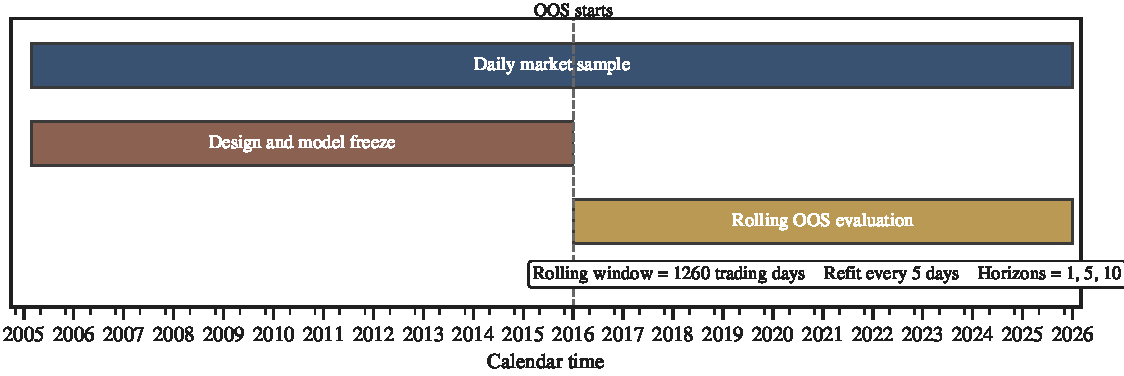
\includegraphics[width=0.96\textwidth]{figures/fig09_protocol_timeline.pdf}
\caption{Rolling walk-forward evaluation protocol. Each step advances the forecast origin by one trading day. The training window (1260 days, shaded) rolls forward to generate the out-of-sample forecast sequence spanning 2016--2025. All feature construction, model fitting, warning-threshold calibration, and evaluation are performed strictly within the boundary of each training window, ensuring full causal integrity.}
\label{fig:protocol_timeline}
\end{figure}

Figure~\ref{fig:protocol_timeline} illustrates the rolling evaluation structure. The causality requirement applies to the full pipeline, not only to the final model fit. Feature standardization, clipping rules, wavelet decomposition, threshold estimation, calibration floors, and warning thresholds are all computed strictly within the current training window. No full-sample preprocessing is used at any stage. This point is crucial because modest-looking violations of chronology, especially in feature construction or normalization, can materially exaggerate out-of-sample performance in financial machine-learning studies.

\subsection{Forecast Horizons, Benchmarks, and Evaluation Metrics}

The main forecast horizons are \(h=1\), \(h=5\), and \(h=10\), corresponding to one trading day, one trading week, and approximately two trading weeks. These horizons separate the short-run persistence problem from the medium-horizon risk-monitoring problem. If a proposed method cannot compete at \(h=1\), that is informative. If it becomes more competitive at \(h=5\) and \(h=10\), that suggests it is capturing slower-moving structure that HAR alone cannot fully absorb.

The benchmark set is intentionally demanding. It includes naive historical-volatility baselines, HAR, raw LightGBM, and wavelet-enhanced LightGBM, as well as the spillover-augmented extension. Additional machine-learning and deep-learning baselines are included so that any performance gain can be attributed to multiscale feature design rather than to model capacity alone.

The primary regression metric is QLIKE because it is widely used in volatility forecasting and is sensitive to both prediction error and scale miscalibration for positive targets \cite{patton2011proxy}. RMSE, MAE, and out-of-sample \(R^2\) are reported as supporting metrics. The out-of-sample coefficient of determination is defined as
\[
R^2_{OOS}
=
1-
\frac{\sum_t (y_t-\hat y_t)^2}
{\sum_t (y_t-\hat y_t^{\,bench})^2}.
\]
For the warning task, PR-AUC is the primary metric because the high-volatility class is intentionally rare under the rolling 90th-percentile rule. ROC-AUC, Brier score, precision, and recall are reported as complementary measures. The Brier score is
\[
\text{Brier}
=
\frac{1}{T}\sum_{t=1}^{T}(p_t-z_t)^2,
\]
where \(p_t\) is the predicted warning probability and \(z_t\) is the realized event label. The threshold-dependent warning quantities are
\[
\text{Precision}(c)=\frac{TP(c)}{TP(c)+FP(c)},
\qquad
\text{Recall}(c)=\frac{TP(c)}{TP(c)+FN(c)},
\]
and
\[
F_{\beta}(c)=
\frac{(1+\beta^2)\,\text{Precision}(c)\,\text{Recall}(c)}
{\beta^2\,\text{Precision}(c)+\text{Recall}(c)}.
\]
The operating threshold for the logistic warning model is chosen by maximizing \(F_2\), reflecting the fact that missed high-volatility episodes are typically more costly than additional false alarms in applied risk surveillance \cite{saito2015prauc}.

\subsection{Three-Step Ablation Design}
\label{subsec:ablation_design}

The core methodological claim of the paper is evaluated through a three-step ablation ladder:

\begin{description}[leftmargin=2.6em, style=nextline]
\item[Step~1: HAR $\to$ Wavelet-LGB]
This comparison tests whether within-index multiscale representation adds predictive value beyond a strong persistence benchmark. It asks whether scale-specific information from the target index's own history contains useful signal beyond the standard 1-, 5-, and 22-day persistence aggregates.

\item[Step~2: Wavelet-LGB $\to$ Spillover-LGB]
This is the central test of the Cross-Index Wavelet Spillover Hypothesis. The only difference between the two models is the addition of the spillover block \(\bm{\phi}_{k\to i,t}\). Any improvement observed here is therefore attributable specifically to peer-index frequency-domain information.

\item[Full gap: HAR $\to$ Spillover-LGB]
This comparison summarizes the cumulative effect of moving from a pure persistence benchmark to the full CMWSL representation.
\end{description}

The value of this ladder is that it prevents the paper from making vague claims about hybrid modelling. Each modelling increment has an identifiable information interpretation: persistence, within-index multiscale representation, and cross-index spillover.

\subsection{Statistical Inference}

Each index--horizon cell is evaluated with explicit out-of-sample forecast comparison tests. The Diebold--Mariano (DM) test is used for non-nested comparisons \cite{diebold1995predictive}. The Clark--West (CW) test is used as the primary inferential tool when the larger model nests the smaller one \cite{clark2007nested}. In the present design, Step~1 is treated with DM because the comparison is conceptually between different representation families, while Step~2 is explicitly nested and therefore primarily evaluated with CW. Reporting both tests increases transparency, but CW is the correct test for the spillover claim because it adjusts for the parameter-estimation noise introduced by the extra regressors.

The DM test is implemented as a two-tailed Newey--West HAC procedure with lag \(\lfloor T^{1/3}\rfloor\). The CW test is implemented one-tailed with the larger model as model \(b\), matching the directional hypothesis that spillover information should improve, rather than simply alter, predictive performance. The nine index--horizon cells are reported separately. No multiple-testing correction is imposed because the spillover analysis is not presented as an exploratory search over arbitrary cells; it is a pre-specified directional test with full cell-level disclosure in Table~\ref{tab:spillover_ablation}.

\subsection{Robustness Strategy}

Two robustness designs are used to test whether the main findings survive beyond one carefully selected benchmark environment. The first augments the predictor set with a broader block of public risk indicators---credit spreads, policy uncertainty variables, and term-structure signals---asking whether multiscale representation becomes more useful in a richer, stress-aligned environment. The second substitutes the Parkinson estimator for the Rogers--Satchell target, asking whether model rankings change when the volatility proxy draws more heavily on OHLC range information.

Together, these designs provide a stronger standard than a single-sample comparison. A method that performs well only under one volatility proxy and one feature set is difficult to generalize. A method whose relative advantage becomes visible precisely when the information environment is richer, or when the target contains stronger OHLC range information, offers a more credible contribution to risk forecasting.


\section{Results}\label{sec:results}
The results are organized around the central empirical question of the paper: under what conditions does CMWSL add predictive value beyond strong persistence benchmarks? Read in that way, the evidence is coherent across all experiments. Three patterns recur. First, one-day index volatility is strongly persistence-driven, and HAR remains the benchmark that must be taken seriously. Second, the value of multiscale representation rises as the task becomes less myopic, the information set becomes richer, or the volatility target contains more informative OHLC structure. Third, cross-index spillover gains are not uniform; they are concentrated in broad-market stress states and in the upper part of the volatility distribution. The section therefore starts with conditional diagnostics, then turns to average performance, robustness designs, risk-warning evidence, the spillover ablation, and interpretability checks.

\subsection{Conditional Evidence Before Average Rankings}

\begin{figure}[!t]
\centering
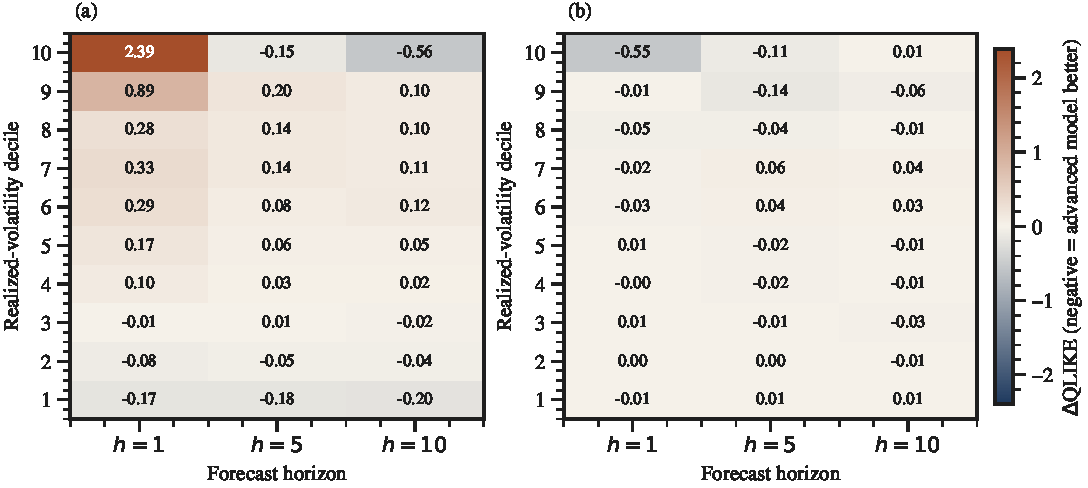
\includegraphics[width=0.96\textwidth]{figures/fig13_quantile_conditioned_delta.pdf}
\caption{Quantile-conditioned $\Delta$QLIKE surfaces. Panel (a) reports Wavelet-LightGBM minus HAR averaged across all indices in the full 2016--2025 package. Panel (b) reports Spillover-LGB minus Wavelet-LGB for the pooled DJIA and S\&P 500 spillover package. Negative values indicate that the more advanced model improves accuracy.}
\label{fig:quantile_conditioned_delta}
\end{figure}

Figure~\ref{fig:quantile_conditioned_delta} shows why the paper should not be read as a simple mean-rank comparison. Panel~(a) indicates that the multiscale model does not improve monotonically over HAR as realized volatility rises. Instead, its advantage is strongest in the calmest deciles and again in the most turbulent decile, while HAR remains strongest in the middle range where volatility is persistent but not yet severely stressed. This U-shaped pattern is economically interpretable. When the market is in a routine regime, short-horizon persistence remains hard to beat. When the market becomes extremely calm or clearly stressed, however, richer scale-specific information becomes more useful. Panel~(b) reveals a parallel result for spillover. The gain from adding peer-index wavelet features is concentrated in the upper volatility deciles, especially at \(h=1\) and \(h=5\), which is consistent with a state-dependent transmission mechanism rather than a uniform cross-market effect.

\begin{figure}[!t]
\centering
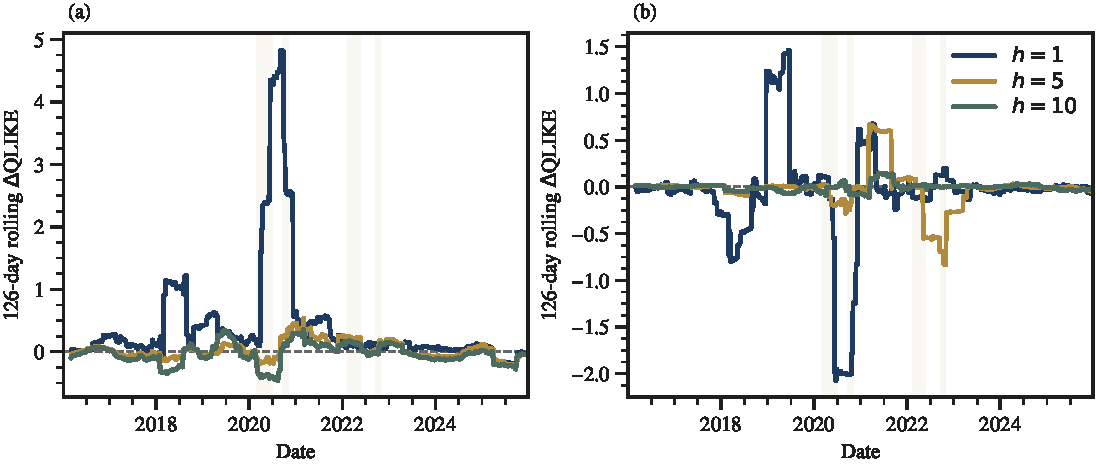
\includegraphics[width=0.96\textwidth]{figures/fig15_timevarying_gain_paths.pdf}
\caption{Time-varying gain paths based on 126-day rolling average $\Delta$QLIKE. Panel (a) reports Wavelet-LGB minus HAR averaged across all indices in the full 2016--2025 package. Panel (b) reports Spillover-LGB minus Wavelet-LGB for the pooled DJIA and S\&P 500 spillover package. Negative values indicate that the more advanced model improves accuracy. Shaded regions denote pooled top-decile VIX stress windows.}
\label{fig:timevarying_gain_paths}
\end{figure}

Figure~\ref{fig:timevarying_gain_paths} shows that the same pattern persists in calendar time. In the pooled 126-day rolling comparison, Wavelet-LGB stays below HAR in only \(8.1\%\) of the \(h=1\) windows, but this share rises to \(50.7\%\) at \(h=5\) and \(59.0\%\) at \(h=10\). The horizon effect is therefore not an artefact of full-sample averaging; it becomes more stable as the target moves away from the one-day persistence problem. Panel~(b) adds the spillover perspective: Spillover-LGB stays below the within-index wavelet model in \(66.8\%\), \(55.7\%\), and \(50.0\%\) of the broad-market rolling windows at \(h=1\), \(h=5\), and \(h=10\), respectively, with the clearest advantages clustered around the 2020 and 2022 stress windows. These diagnostics justify the central framing of the paper: the value of CMWSL is conditional, and those conditions align with economically meaningful market states.

\subsection{Main Forecasting Results: Strong Benchmark, Narrow Margins}

\begin{table}[!t]
\caption{Main regression QLIKE across indices and forecast horizons under the Rogers--Satchell target. Best, second-best, and third-best values within each index--horizon cell are marked by \best{bold shading}, \second{underline}, and \third{light shading}, respectively.}
\label{tab:main_regression}
\centering
\small
\setlength{\tabcolsep}{6pt}
\renewcommand{\arraystretch}{1.12}
\begin{tabular}{llccc}
\toprule
Index & Model & $h=1$ & $h=5$ & $h=10$ \\
\midrule
S\&P 500 & HAR & \best{-9.0316} & \best{-8.9372} & \second{-8.8682} \\
 & HV-22 & \second{-8.9405} & -8.8601 & -8.7836 \\
 & LightGBM & \third{-8.7386} & \second{-8.9022} & \best{-8.8749} \\
 & Wavelet-LightGBM & -8.7327 & \third{-8.8937} & \third{-8.8603} \\
\midrule
Nasdaq-100 & HAR & \best{-8.5635} & \third{-8.4940} & \third{-8.4316} \\
 & HV-22 & \second{-8.5049} & -8.4472 & -8.3873 \\
 & LightGBM & \third{-8.4476} & \best{-8.5125} & \second{-8.4621} \\
 & Wavelet-LightGBM & -8.3827 & \second{-8.5026} & \best{-8.4923} \\
\midrule
DJIA & HAR & \best{-9.0021} & \best{-8.9139} & \third{-8.8548} \\
 & HV-22 & \second{-8.9398} & \third{-8.8619} & -8.7869 \\
 & LightGBM & \third{-8.5186} & -8.8111 & \second{-8.8636} \\
 & Wavelet-LightGBM & -8.2222 & \second{-8.8649} & \best{-8.8934} \\
\bottomrule
\end{tabular}
\end{table}


\begin{figure}[!t]
\centering
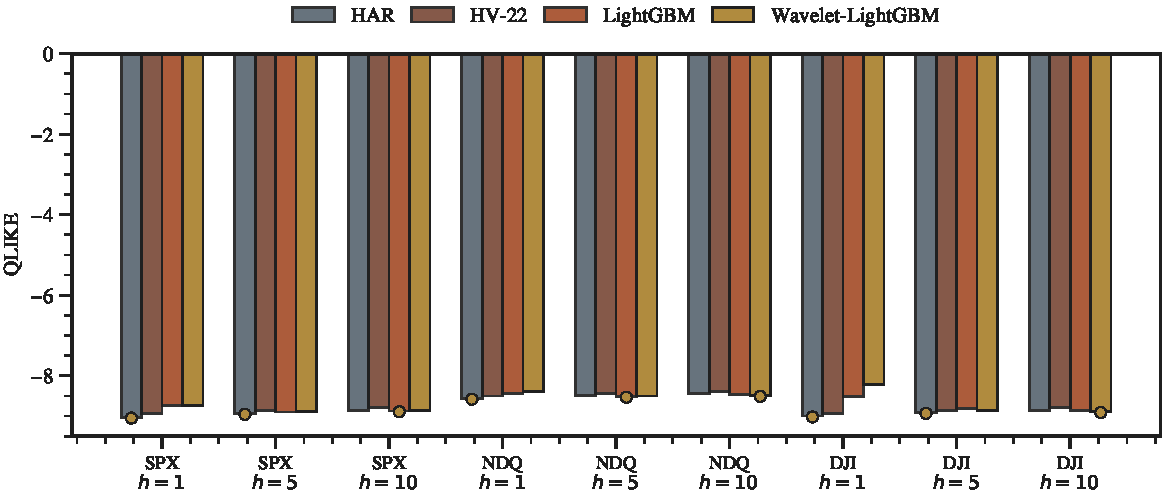
\includegraphics[width=0.98\textwidth]{figures/fig02_main_qlike_bars.pdf}
\caption{QLIKE across indices and forecast horizons in the main Rogers--Satchell specification. Lower values indicate better performance.}
\label{fig:main_qlike_bars}
\end{figure}

\begin{figure}[!t]
\centering
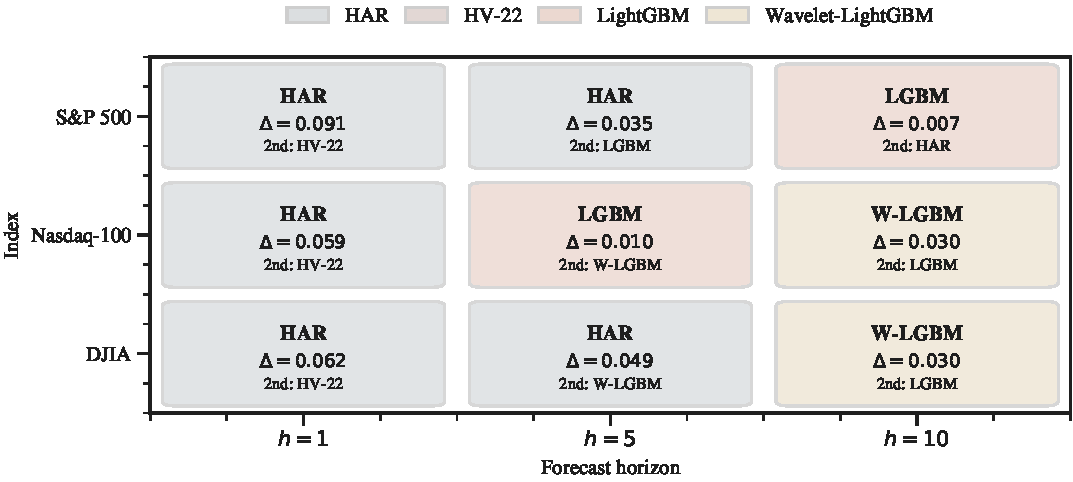
\includegraphics[width=0.98\textwidth]{figures/fig03_main_qlike_heatmap.pdf}
\caption{Winner-and-margin map for the main Rogers--Satchell specification. Each tile reports the winner and its QLIKE margin over the runner-up.}
\label{fig:main_qlike_heatmap}
\end{figure}

Table~\ref{tab:main_regression} and Figures~\ref{fig:main_qlike_bars}--\ref{fig:main_qlike_heatmap} establish the baseline difficulty of the forecasting problem. In the main Rogers--Satchell specification, HAR remains the best average model on QLIKE, with an average value of \(-8.789\), compared with \(-8.724\) for HV-22, \(-8.681\) for raw LightGBM, and \(-8.649\) for \textit{wavelet\_lightgbm}. This is a substantive result rather than a negative one. It confirms that daily stock-index volatility remains dominated by persistence, and that any paper claiming strong performance gains should be judged against that fact.

At the cell level, however, the picture is more nuanced. HAR wins five of the nine index--horizon contests, while LightGBM and \textit{wavelet\_lightgbm} each win two. The multiscale model is strongest for DJIA at \(h=10\) and Nasdaq-100 at \(h=10\), while raw LightGBM wins Nasdaq-100 at \(h=5\) and S\&P~500 at \(h=10\). Figure~\ref{fig:main_qlike_heatmap} is especially informative because it shows that several medium- and longer-horizon contests are narrow even when HAR remains the formal winner. The main sample should therefore be interpreted as showing two things simultaneously: short-horizon persistence is extremely hard to beat, but multiscale representation becomes meaningfully competitive once the horizon lengthens.

\subsection{Richer Public Information Strengthens the Multiscale Design}

\begin{table}[!t]
\caption{Average QLIKE across the main and robustness settings. Ranking is applied within each row.}
\label{tab:robustness_summary}
\centering
\small
\setlength{\tabcolsep}{6pt}
\renewcommand{\arraystretch}{1.12}
\begin{tabular}{lccc}
\toprule
Setting & HAR & LightGBM & Wavelet-LightGBM \\
\midrule
Main RS & \best{-8.7885} & \second{-8.6812} & \third{-8.6494} \\
Expanded Data & \best{-9.5949} & \third{-9.5641} & \second{-9.5704} \\
Parkinson & \third{-9.3019} & \second{-9.3091} & \best{-9.3143} \\
\bottomrule
\end{tabular}
\end{table}


\begin{figure}[!t]
\centering
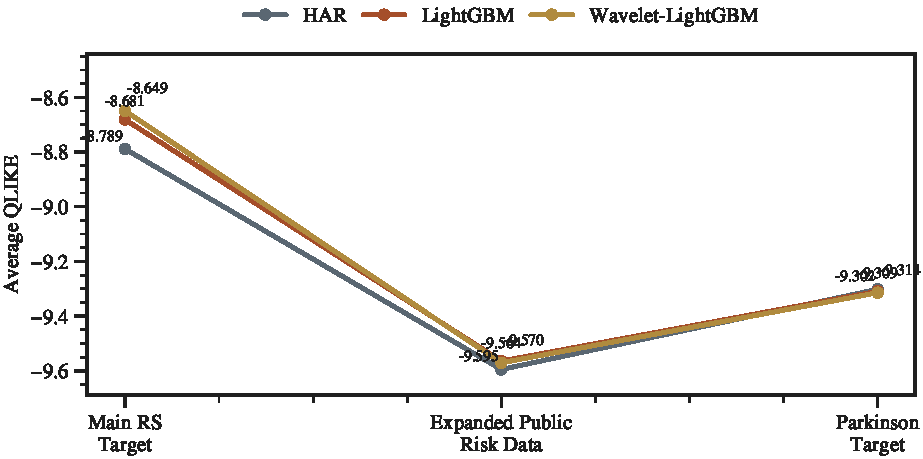
\includegraphics[width=0.94\textwidth]{figures/fig04_robustness_comparison.pdf}
\caption{Average QLIKE across the main and robustness settings. Lower values indicate better performance.}
\label{fig:robustness_comparison}
\end{figure}

\begin{figure}[!t]
\centering
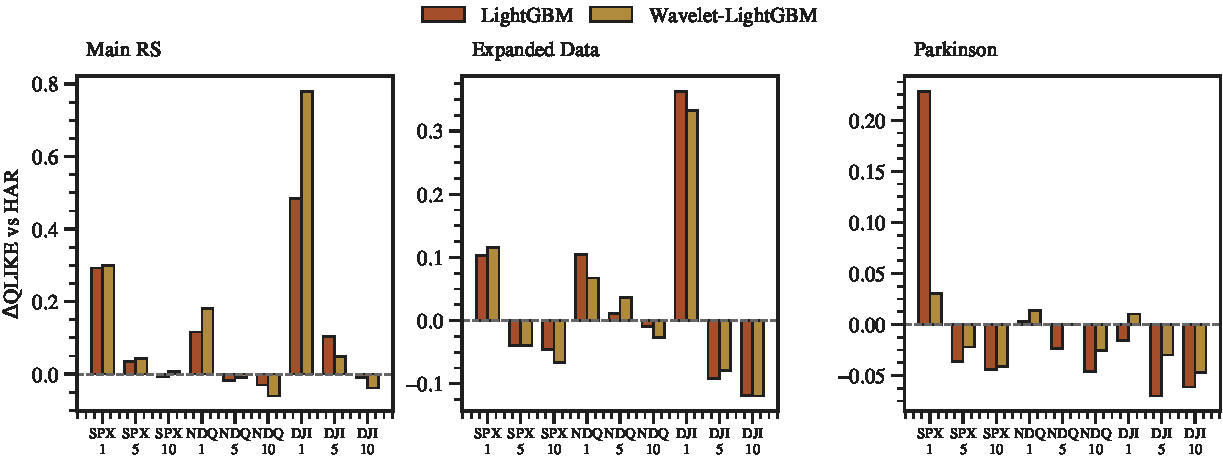
\includegraphics[width=0.94\textwidth]{figures/fig07_delta_vs_har.pdf}
\caption{Cell-level QLIKE differences relative to HAR. Negative values indicate that the nonlinear model outperforms HAR.}
\label{fig:delta_vs_har}
\end{figure}

The expanded public-information setting provides stronger support for CMWSL. After adding public credit-spread, policy-uncertainty, and volatility-term-structure variables, the average QLIKE of \textit{wavelet\_lightgbm} improves to \(-9.570\), much closer to HV-22 \((-9.618)\) and HAR \((-9.595)\). In this richer environment, the multiscale model wins four of the nine index--horizon cells, including DJIA at \(h=10\), Nasdaq-100 at \(h=10\), and S\&P~500 at both \(h=5\) and \(h=10\). This shift is central to the paper's interpretation. It suggests that the wavelet layer is not merely fitting noise in the main sample; it becomes more useful precisely when the public information set contains broader market-risk content that benefits from multiscale organization.

Figures~\ref{fig:robustness_comparison} and~\ref{fig:delta_vs_har} reinforce this interpretation. The comparison against HAR improves not only on average, but also in the cell-by-cell pattern. Appendix Figure~\ref{fig:forecast_panels_appendix} shows the same effect in time-series traces: isolated spikes still often favor HAR, but the wavelet-enhanced model tracks stress build-up and normalization more smoothly at \(h=5\) and \(h=10\). Appendix Figures~\ref{fig:multiscale_signal_heatmap_appendix} and~\ref{fig:block_contribution_heatmap_appendix} further indicate that the strongest associations with future volatility lie in longer-scale detail components and that macro-financial information becomes the most useful feature block once the public-information panel is expanded.

\subsection{Alternative Target and Risk-Warning Evidence}

The Parkinson robustness experiment sharpens the same message. Under this alternative OHLC target, \textit{wavelet\_lightgbm} achieves the best average QLIKE at \(-9.314\), slightly outperforming LightGBM \((-9.309)\) and HAR \((-9.302)\). The raw boosting model still wins five of the nine cells, so the result should not be overstated. But the average lead of the wavelet model is important because it indicates that CMWSL is more useful when the target itself contains richer range information than in the baseline Rogers--Satchell setting.

\begin{table}[!t]
\caption{Main warning results under the Rogers--Satchell target. PR-AUC is maximized and Brier score is minimized within each index--horizon cell.}
\label{tab:warning_results}
\centering
\small
\setlength{\tabcolsep}{5.2pt}
\renewcommand{\arraystretch}{1.12}
\begin{tabular}{llcccccc}
\toprule
Index & Model & PR$(1)$ & Brier$(1)$ & PR$(5)$ & Brier$(5)$ & PR$(10)$ & Brier$(10)$ \\
\midrule
S\&P 500 & Naive Threshold & \second{0.4895} & \best{0.0948} & \second{0.5041} & \best{0.0985} & \second{0.4474} & \best{0.1041} \\
 & Logistic-Raw & \best{0.5275} & \second{0.1327} & \best{0.5048} & \second{0.1271} & \best{0.5530} & \second{0.1143} \\
\midrule
Nasdaq-100 & Naive Threshold & \second{0.4652} & \best{0.1072} & \second{0.5141} & \best{0.1090} & \second{0.4496} & \best{0.1148} \\
 & Logistic-Raw & \best{0.5496} & \second{0.1418} & \best{0.5960} & \second{0.1258} & \best{0.4852} & \second{0.1399} \\
\midrule
DJIA & Naive Threshold & \second{0.4733} & \best{0.0954} & \second{0.4882} & \best{0.0972} & \best{0.4712} & \best{0.0998} \\
 & Logistic-Raw & \best{0.4900} & \second{0.1402} & \best{0.5782} & \second{0.1069} & \second{0.4672} & \second{0.1112} \\
\bottomrule
\end{tabular}
\end{table}


\begin{figure}[!t]
\centering
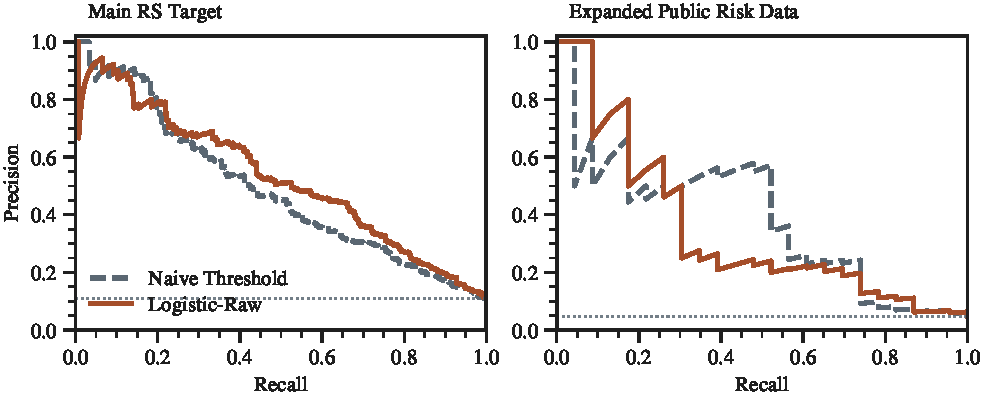
\includegraphics[width=0.94\textwidth]{figures/fig06_warning_pr_panels.pdf}
\caption{Precision--recall comparison for the warning task using the S\&P 500 at \(h=1\).}
\label{fig:warning_panels}
\end{figure}

\begin{figure}[!t]
\centering
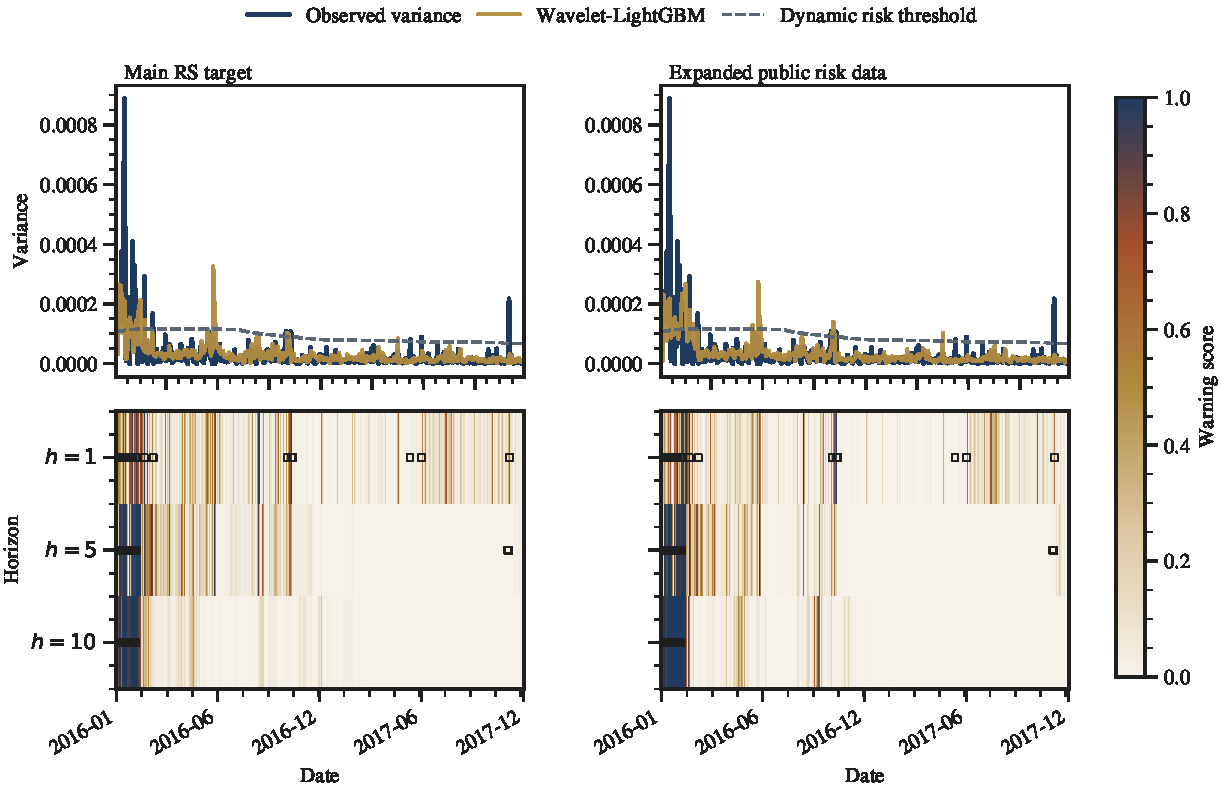
\includegraphics[width=0.94\textwidth]{figures/fig08_warning_score_distribution.pdf}
\caption{Event-aligned warning diagnostics for the S\&P 500 during the 2020 stress period.}
\label{fig:warning_score_distribution}
\end{figure}

\begin{table}[!t]
\caption{Event-based warning timing summary using a five-day pre-event detection window. Hit rate and median lead are maximized; false-alarm days per event are minimized within each horizon.}
\label{tab:warning_event_timing}
\centering
\footnotesize
\setlength{\tabcolsep}{4.6pt}
\renewcommand{\arraystretch}{1.12}
\begin{tabular}{llcccc}
\toprule
Horizon & Model & Hit rate & Median lead & FA / event & Events \\
\midrule
$h=1$ & Logistic-Raw & \best{0.821} & \best{5.000} & 5.149 & 460 \\
 & Naive-Threshold & 0.613 & 4.000 & \best{1.005} & 460 \\
\midrule
$h=5$ & Logistic-Raw & 0.597 & \best{5.000} & 16.558 & 134 \\
 & Naive-Threshold & \best{0.649} & 3.833 & \best{3.641} & 134 \\
\midrule
$h=10$ & Logistic-Raw & \best{0.602} & \best{5.000} & 37.330 & 81 \\
 & Naive-Threshold & 0.556 & 4.333 & \best{6.463} & 81 \\
\bottomrule
\end{tabular}
\end{table}


For the risk early-warning task, the clearest evidence comes from the interpretable logistic classifier estimated on raw market-risk features. In the main specification, \textit{logistic\_raw} reaches an average PR-AUC of \(0.528\), compared with \(0.478\) for the naive threshold rule, and also achieves a higher average ROC-AUC. In the expanded public-information setting, its PR-AUC rises further to \(0.593\), again the strongest result among the warning models. Under the Parkinson target, \textit{logistic\_raw} remains the top model on PR-AUC at \(0.559\). Figure~\ref{fig:warning_panels} makes this ranking visible in precision--recall space, while Figure~\ref{fig:warning_score_distribution} shows that elevated warning scores cluster around realized high-volatility episodes rather than appearing uniformly through time.

Table~\ref{tab:warning_event_timing} shows that warning quality should also be interpreted as a timing problem. Using a five-day pre-event detection window, \textit{logistic\_raw} detects a larger share of events than the threshold rule at \(h=1\) and \(h=10\) and also provides longer median lead times. The price is a higher alert burden, measured by false-alarm days per event. At \(h=5\), the threshold rule remains more economical and slightly stronger on hit rate. The practical implication is that the logistic warning model is more aggressive and earlier, whereas the threshold rule is sparser and more conservative. Appendix Figure~\ref{fig:warning_event_frontier_appendix} visualizes this operating frontier at the index--horizon level.

Full DM and CW benchmark-comparison tests are reported in Appendix Table~\ref{tab:significance_tests}. The overall message remains disciplined: there is no blanket nonlinear dominance, but there is clear evidence that incremental predictive content appears when the horizon lengthens, the information set broadens, or the market enters more stressed states.

\subsection{Cross-Index Spillover Ablation Results}
\label{subsec:results_spillover}

Table~\ref{tab:spillover_ablation} reports the full three-step ablation evidence over the 2016--2025 out-of-sample evaluation. This is the most direct test of the paper's novelty claim because it asks whether peer-index frequency-domain information adds value beyond within-index multiscale representation.

\begin{table}[!t]
\caption{Three-step ablation test results. Columns report mean QLIKE for each model, the
Diebold--Mariano statistic and p-value for Step~1 (HAR vs.\ Wavelet-LGB) and Step~2
(Wavelet-LGB vs.\ Spillover-LGB), and the Clark--West statistic and p-value for the
nested Step-2 comparison. DM tests are two-tailed with Newey-West HAC; CW test is
one-tailed (Ho:\ spillover carries no incremental information). Significance codes:
${}^{***}p<0.001$, ${}^{**}p<0.01$, ${}^{*}p<0.05$, ${}^{.}p<0.10$.
QLIKE convention: lower values indicate better forecasting accuracy.}
\label{tab:spillover_ablation}
\centering
\small
\setlength{\tabcolsep}{4pt}
\renewcommand{\arraystretch}{1.12}
\resizebox{\textwidth}{!}{%
\begin{tabular}{llccc  cc  cc  cc}
\toprule
 & & \multicolumn{3}{c}{Mean QLIKE} &
   \multicolumn{2}{c}{Step 1 DM} &
   \multicolumn{2}{c}{Step 2 DM} &
   \multicolumn{2}{c}{Step 2 CW (nested)} \\
\cmidrule(lr){3-5}\cmidrule(lr){6-7}\cmidrule(lr){8-9}\cmidrule(lr){10-11}
Index & $h$ & HAR & Wav-LGB & Spill-LGB &
  $t_{\!DM}$ & $p$ &
  $t_{\!DM}$ & $p$ &
  $t_{\!CW}$ & $p$ \\
\midrule
DJIA & $h=1$ & $-9.0021$ & $-8.1817$ & $-8.2476$ & $-3.666$ & $0.0002^{***}$ & $0.317$ & $0.7515$ & $1.749$ & $0.0401^{*}$ \\
 & $h=5$ & $-8.9139$ & $-8.6564$ & $-8.7303$ & $-2.356$ & $0.0185^{*}$ & $1.427$ & $0.1536$ & $2.613$ & $0.0045^{**}$ \\
 & $h=10$ & $-8.8548$ & $-8.9037$ & $-8.8932$ & $1.522$ & $0.1280$ & $-0.812$ & $0.4166$ & $1.394$ & $0.0816^{.}$ \\
\midrule
Nasdaq-100 & $h=1$ & $-8.5635$ & $-8.2771$ & $-8.2892$ & $-4.881$ & $<0.0001^{***}$ & $0.207$ & $0.8363$ & $0.293$ & $0.3847$ \\
 & $h=5$ & $-8.4940$ & $-8.5154$ & $-8.5027$ & $1.308$ & $0.1909$ & $-0.983$ & $0.3256$ & $-1.521$ & $0.9358$ \\
 & $h=10$ & $-8.4316$ & $-8.5149$ & $-8.5103$ & $3.417$ & $0.0006^{***}$ & $-0.625$ & $0.5318$ & $0.977$ & $0.1644$ \\
\midrule
S\&P~500 & $h=1$ & $-9.0316$ & $-8.8211$ & $-8.8841$ & $-2.637$ & $0.0084^{**}$ & $1.353$ & $0.1761$ & $2.077$ & $0.0189^{*}$ \\
 & $h=5$ & $-8.9372$ & $-8.8741$ & $-8.8444$ & $-1.046$ & $0.2957$ & $-0.548$ & $0.5838$ & $1.945$ & $0.0259^{*}$ \\
 & $h=10$ & $-8.8682$ & $-8.8970$ & $-8.9141$ & $0.772$ & $0.4402$ & $1.199$ & $0.2307$ & $4.827$ & $<0.0001^{***}$ \\
\bottomrule
\end{tabular}
}
\end{table}


\begin{figure}[!t]
\centering
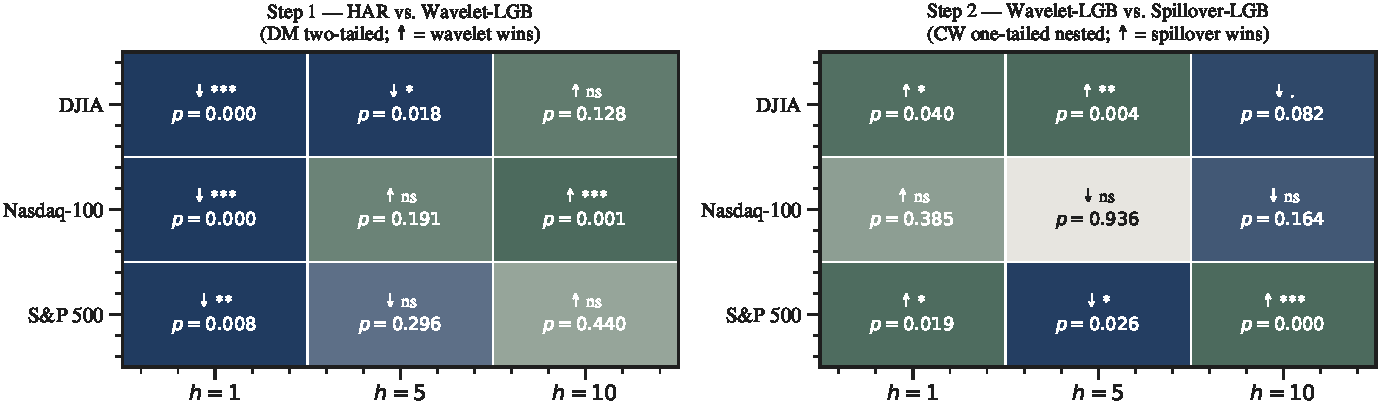
\includegraphics[width=0.94\textwidth]{figures/fig_spillover_cw_heatmap.pdf}
\caption{Statistical evidence heatmap for each ablation step.
  Left: Diebold--Mariano two-tailed test for Step~1 (HAR vs.\ Wavelet-LGB).
  Right: Clark--West one-tailed test for Step~2 (Wavelet-LGB vs.\ Spillover-LGB).
  Teal tones indicate that the advanced model wins at the stated significance level;
  navy tones indicate the simpler model wins.
  Colour intensity scales with $1-p$.}
\label{fig:spillover_cw_heatmap}
\end{figure}

\begin{figure}[!t]
\centering
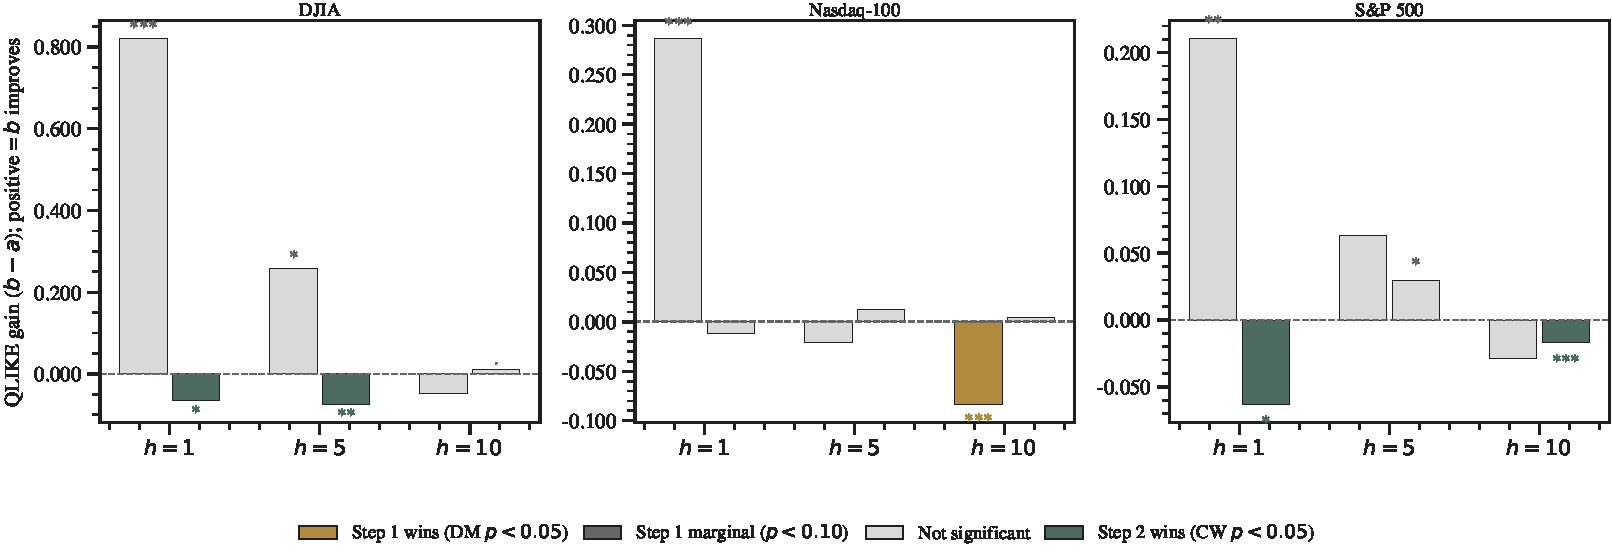
\includegraphics[width=0.94\textwidth]{figures/fig_spillover_gain_ladder.pdf}
\caption{QLIKE gain ladder per index.
  Each panel shows the incremental QLIKE gain (positive = improvement over baseline)
  for Step~1 (amber bars when DM-significant, light grey otherwise) and
  Step~2 (teal bars when CW-significant, light grey otherwise).
  Significance codes: ${}^{***}p<0.001$, ${}^{**}p<0.01$, ${}^{*}p<0.05$, ${}^{.}p<0.10$.}
\label{fig:spillover_gain_ladder}
\end{figure}

\paragraph{Step~1: HAR versus within-index wavelet representation.}
The first ablation step shows that within-index wavelet features add value selectively rather than uniformly. For DJIA, HAR significantly outperforms Wavelet-LGB at \(h=1\) (DM \(t=-3.67\), \(p<0.001\)) and \(h=5\) (\(p=0.019\)), confirming that short-run persistence dominates for this broad, price-weighted index. The relative advantage narrows at \(h=10\), where Wavelet-LGB posts a slightly better QLIKE, though not significantly so. For Nasdaq-100, HAR dominates strongly at \(h=1\) (DM \(t=-4.88\), \(p<0.001\)), but the relation reverses at \(h=10\) (\(p=0.001\)), indicating richer long-horizon multiscale structure in the technology-heavy index. For S\&P~500, HAR wins significantly at \(h=1\), while the medium- and long-horizon cells are statistically inconclusive. Step~1 therefore supports the first part of the paper's argument: wavelet representation is most useful when the problem moves away from the one-day persistence regime.

\paragraph{Step~2: within-index wavelet versus spillover-augmented wavelet.}
The second ablation step is the core test of the Cross-Index Wavelet Spillover Hypothesis. The two-sided DM test does not reach \(p<0.05\) in any of the nine cells, which is not surprising in a nested setting where the larger model pays an estimation-noise penalty. The CW test, which is specifically designed for nested comparisons, paints a more informative picture.

Five of the nine cells are significant at \(p<0.05\) under CW. DJIA shows significant gains at \(h=1\) (CW \(t=1.75\), \(p=0.040\)) and \(h=5\) (CW \(t=2.61\), \(p=0.005\)). S\&P~500 shows significant gains at \(h=1\) (\(p=0.019\)), \(h=5\) (\(p=0.026\)), and most strongly at \(h=10\) (CW \(t=4.83\), \(p<0.001\)). The S\&P~500 \(h=10\) cell is the clearest positive result in the article: peer-index d2/d3 wavelet energy provides information about future broad-market volatility that is not already contained in the target index's own persistence and multiscale history.

Nasdaq-100 behaves differently. None of its three cells is significant under CW, and the \(h=5\) cell even shows a negative CW statistic. This absence of spillover response is informative in its own right. It suggests that the volatility dynamics of a technology-concentrated index occupy a different frequency-domain regime from those of the broad-market indices used as peers. The same weekly-to-biweekly peer-market channels that help forecast DJIA and S\&P~500 do not transfer cleanly to Nasdaq-100.

The regime-conditioned evidence in Appendix Table~\ref{tab:spillover_regime} sharpens this interpretation. For the pooled DJIA and S\&P~500 sample, spillover gains are strongest in recession and high-VIX windows at \(h=1\) and \(h=5\). Combined with Figures~\ref{fig:quantile_conditioned_delta} and~\ref{fig:timevarying_gain_paths}, the result supports a clear interpretation: peer-index wavelet information is most useful when broad-market stress is elevated, synchronized, and still unfolding.

\paragraph{Why DM and CW differ.}
The divergence between DM and CW is not contradictory. DM tests realized loss differences directly and does not correct for the attenuation induced by estimating additional regressors in the larger model. CW adds the usual nested-model adjustment term \((\hat y_{1,t}-\hat y_{2,t})^2\), which raises power when the larger model contains real but noisy incremental information \cite{clark2007nested}. In the present setting, the pattern of positive QLIKE gains combined with CW significance indicates that the spillover features contain useful predictive signal, even though that signal is modest and partially offset by estimation noise in finite rolling samples.

\paragraph{Takeaway from the ablation.}
The spillover ladder establishes three regularities. HAR remains the dominant short-horizon benchmark. Within-index wavelet representation adds value selectively, mainly at longer horizons. Cross-index d2/d3 spillover features provide statistically significant incremental information for DJIA and S\&P~500 at multiple horizons, with the S\&P~500 \(h=10\) cell providing the strongest evidence. This is the most novel result of the paper because it isolates a specific type of cross-market information that matters precisely where time-domain persistence becomes less sufficient.

\subsection{Interpretability and Deep-Learning Benchmarking}
\label{subsec:results_shap}

To examine whether the gains of CMWSL are driven by economically meaningful inputs rather than by opaque tree interactions, we compute SHAP values \cite{lundberg2017shap} for a full-window \textit{wavelet\_lightgbm} model fitted at the start of the test period for the S\&P~500 index at both $h=1$ and $h=5$.

\begin{figure}[!t]
\centering
\subfloat[$h=1$: persistence and short-run signals dominate; wavelet features appear further down.\label{fig:shap_bar_h1}]{%
  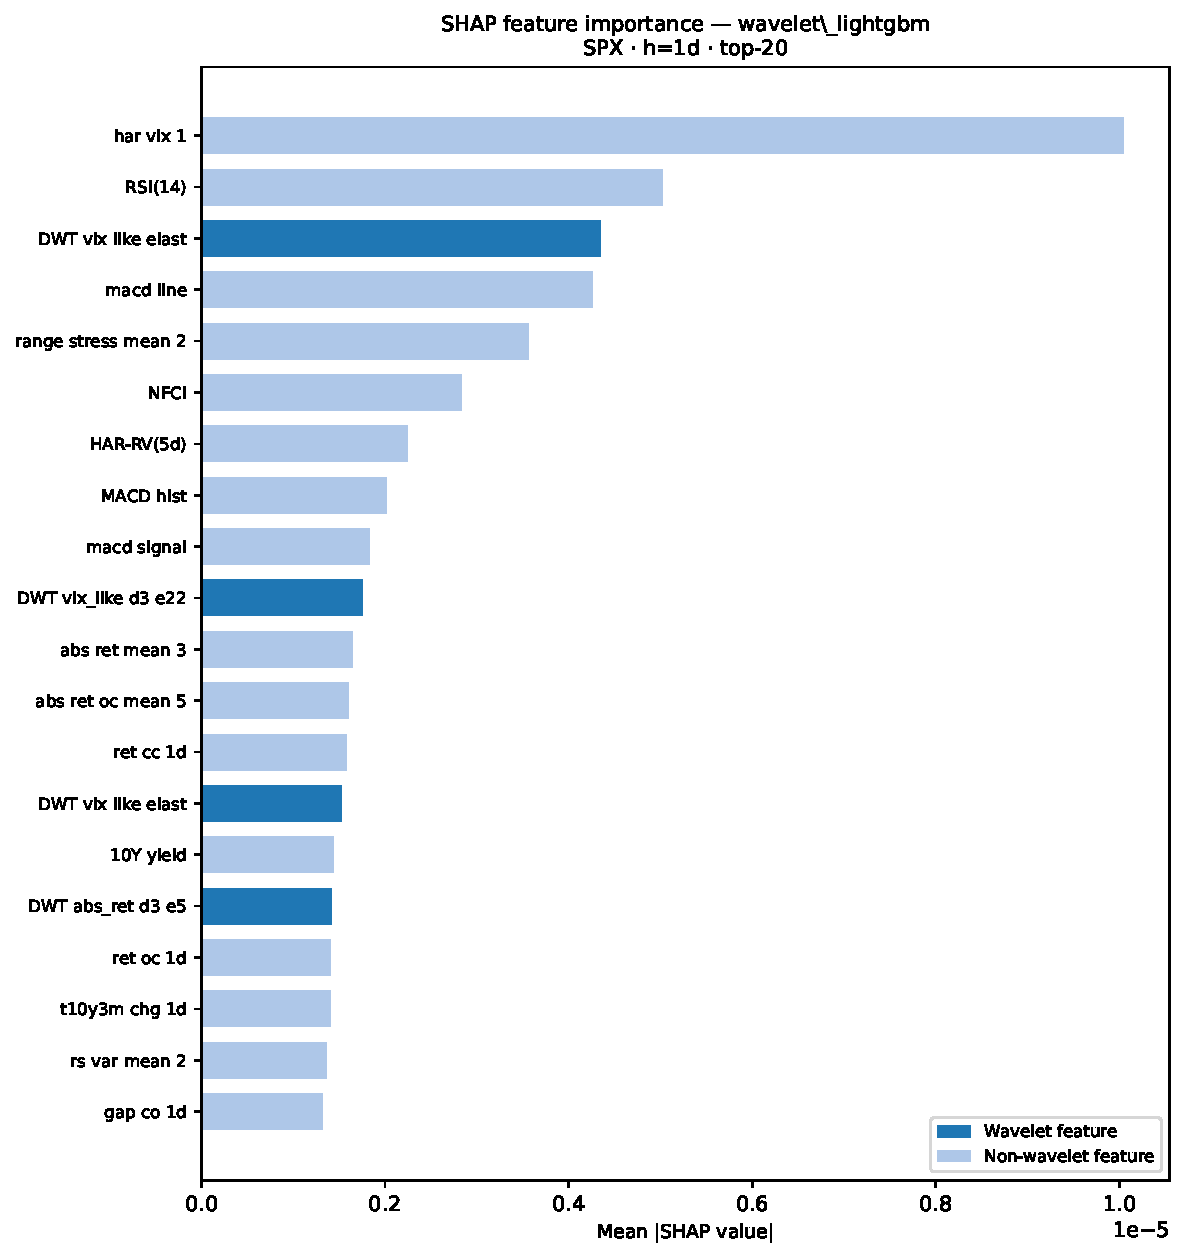
\includegraphics[width=0.47\textwidth]{figures/shap_bar_spx_h1.pdf}}
\hfill
\subfloat[$h=5$: wavelet energy at d2/d3 scales rises sharply in the ranking.\label{fig:shap_bar_h5}]{%
  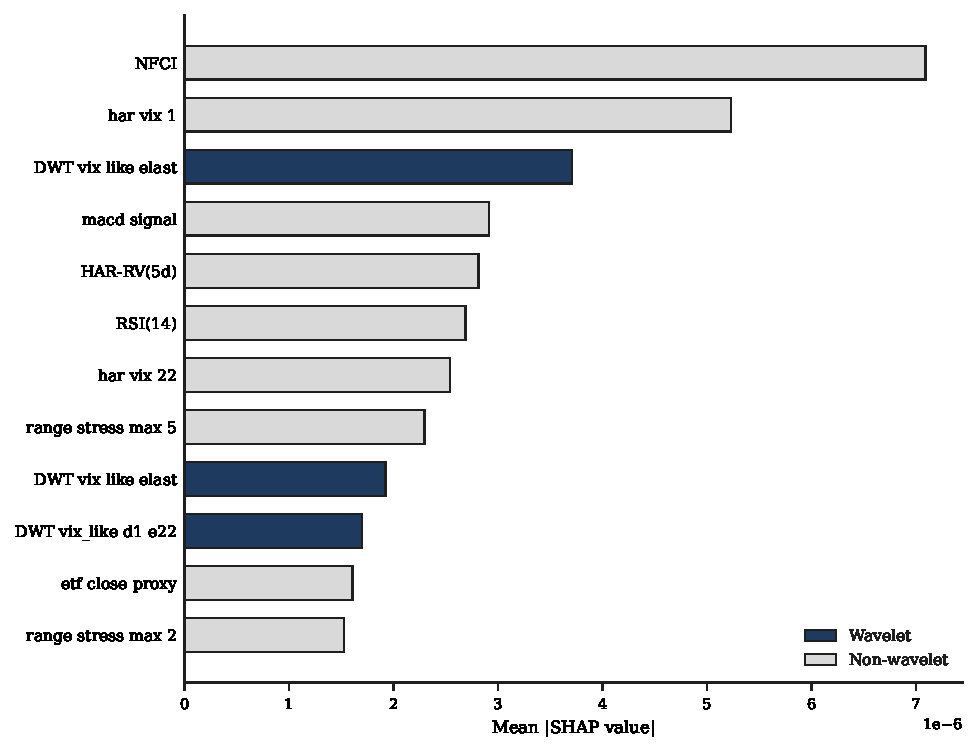
\includegraphics[width=0.47\textwidth]{figures/shap_bar_spx_h5.pdf}}
\caption{Horizon-dependent SHAP feature attribution (top-12 mean absolute values) for \textit{wavelet\_lightgbm} (S\&P~500). Navy bars denote wavelet features; grey bars denote non-wavelet features. The shift from $h=1$ to $h=5$ confirms that medium-scale frequency-domain information adds value selectively as the forecast horizon lengthens---consistent with the quantile-conditioned and rolling-window evidence in Figures~\ref{fig:quantile_conditioned_delta} and~\ref{fig:timevarying_gain_paths}.}
\label{fig:shap_horizon_comparison}
\end{figure}

\begin{figure}[!t]
\centering
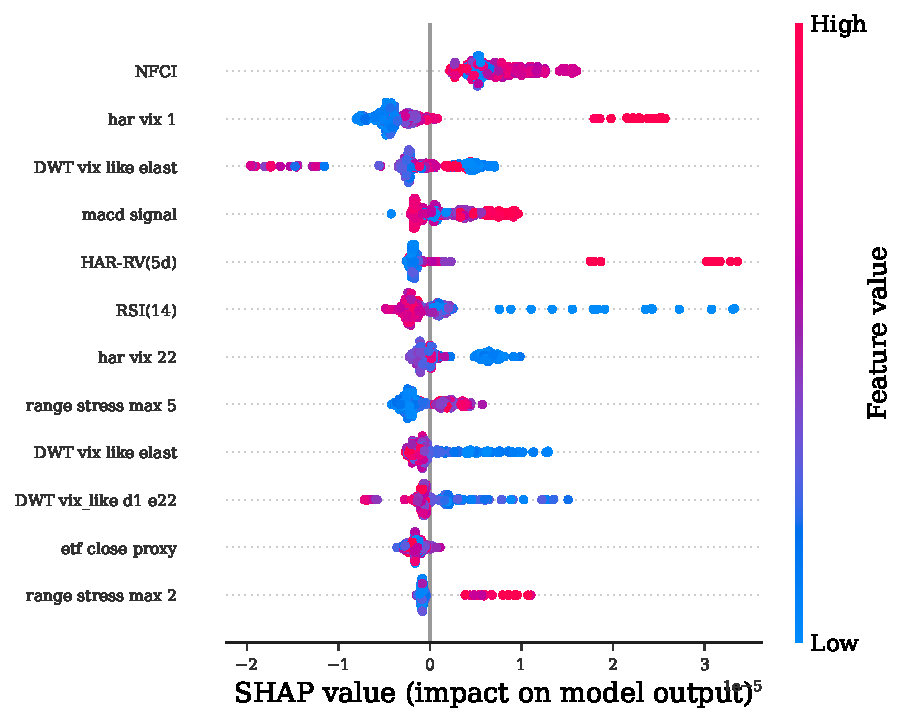
\includegraphics[width=0.60\textwidth]{figures/shap_beeswarm_spx_h5.pdf}
\caption{SHAP beeswarm for \textit{wavelet\_lightgbm} (S\&P~500, $h=5$). Each point is one observation; colour encodes the feature value. SWT energy features at the d2/d3 decomposition levels rank among the most influential predictors, and high energy values consistently produce positive SHAP contributions, confirming that medium-scale frequency-domain volatility drives upward forecast revisions.}
\label{fig:shap}
\end{figure}

Figure~\ref{fig:shap_horizon_comparison} documents the horizon-dependent shift in feature importance. At $h=1$, HAR persistence lags and short-run technical signals such as MACD and ATR dominate the ranking, consistent with a regime where next-day volatility is primarily determined by the recent level and trajectory of the series. At $h=5$, wavelet energy variables at the d2 and d3 scales of the VIX-related and Rogers--Satchell input series move to the top of the ranking, while the relative importance of raw persistence lags declines. This transition mirrors the pattern documented in Figures~\ref{fig:quantile_conditioned_delta} and~\ref{fig:timevarying_gain_paths}, and directly supports the paper's central interpretation that medium-scale frequency-domain structure becomes decision-relevant precisely as the forecast horizon extends into the range most useful for portfolio risk monitoring.

\subsection{LSTM Baseline Comparison}
\label{subsec:results_dl}

To test whether the performance of \textit{wavelet\_lightgbm} reflects feature quality rather than only model flexibility, we include a compact LSTM baseline evaluated under the same 1260-day rolling protocol. The LSTM is trained on the three HAR inputs, uses 16 hidden units with chronological early stopping, and targets the same log1p-transformed realized variance as the tree-based models. This HAR-LSTM specification asks whether a neural sequence model can extract gains from the standard persistence feature set without the wavelet layer.

\begin{table}[!t]
\caption{QLIKE comparison of benchmark models and the HAR-LSTM deep-learning
baseline under the same 1260-day rolling walk-forward protocol.
The LSTM is trained on the three HAR features (1-, 5-, and 22-day realized
variance) with 16 hidden units and chronological early stopping.
Best value per index--horizon cell is \best{bold-shaded}; second-best is \second{underlined}.}
\label{tab:dl_comparison}
\centering
\small
\setlength{\tabcolsep}{5pt}
\renewcommand{\arraystretch}{1.10}
\begin{tabular}{llccc}
\toprule
Index & Model & $h=1$ & $h=5$ & $h=10$ \\
\midrule
S\&P 500 & HAR & \best{0.5204} & \best{0.3168} & \second{0.3085} \\
  & HV-22 & 0.6122 & 0.3939 & 0.3932 \\
  & LightGBM & 0.8149 & \second{0.3518} & \best{0.3019} \\
  & \textit{wavelet\_lightgbm} & 0.8210 & 0.3603 & 0.3165 \\
\cmidrule(lr){2-5}
  & LSTM & \second{0.6072} & 0.3946 & 0.3510 \\
\midrule
Nasdaq-100 & HAR & \best{0.4798} & 0.2763 & 0.2733 \\
  & HV-22 & 0.5386 & 0.3231 & 0.3176 \\
  & LightGBM & 0.5955 & \best{0.2578} & \second{0.2428} \\
  & \textit{wavelet\_lightgbm} & 0.6607 & \second{0.2677} & \best{0.2126} \\
\cmidrule(lr){2-5}
  & LSTM & \second{0.5176} & 0.3097 & 0.2910 \\
\midrule
DJIA & HAR & \best{0.5169} & \best{0.3144} & 0.3048 \\
  & HV-22 & \second{0.5795} & 0.3665 & 0.3727 \\
  & LightGBM & 1.0023 & 0.4173 & \second{0.2960} \\
  & \textit{wavelet\_lightgbm} & 1.3000 & \second{0.3634} & \best{0.2662} \\
\cmidrule(lr){2-5}
  & LSTM & 0.5957 & 0.3653 & 0.3430 \\
\midrule
\bottomrule
\end{tabular}
\end{table}

Table~\ref{tab:dl_comparison} shows that the LSTM is broadly comparable to HAR at \(h=1\) but remains behind \textit{wavelet\_lightgbm} at \(h\ge 5\), where the multiscale feature advantage is most pronounced. This is important for the paper's interpretation. It indicates that the main contribution of CMWSL is not simply ``nonlinearity''. Rather, it is the design of a causal multiscale and spillover-aware feature space that can then be learned efficiently by a well-calibrated tree model.


\section{Discussion}\label{sec:discussion}
The results support a clear but disciplined interpretation. CMWSL does not overturn the well-known fact that daily stock-index volatility is strongly persistence-driven. HAR remains the right benchmark, and in the main Rogers--Satchell specification it remains the strongest average model. That finding should not be minimized. It is precisely because the benchmark is strong that the conditional gains documented in this paper matter. A credible contribution in this literature is not universal dominance over HAR, but a precise account of when richer representation begins to add value.

The first substantive implication concerns forecast horizon. The results consistently show that the relative value of multiscale representation rises as the task moves from one-day forecasting toward five- and ten-day horizons. This pattern has a natural economic interpretation. At the shortest horizon, the next day's volatility is heavily determined by immediate persistence and local market continuation. At longer horizons, however, medium-scale adjustment processes, information diffusion, and broader market-risk conditions have more time to matter. The wavelet layer is useful precisely because it organizes those medium-scale dynamics without discarding the strong persistence structure already captured by HAR.

The second implication concerns information richness. CMWSL performs more strongly when the predictor set is expanded with public credit-spread, policy-uncertainty, and volatility-term-structure variables, and when the target is changed from Rogers--Satchell to Parkinson volatility. These are not incidental robustness wins. Together they suggest that the multiscale layer becomes more valuable when the forecasting environment contains more heterogeneous information or when the target places more weight on informative OHLC range variation. In other words, the wavelet design is not acting as a generic complexity booster; it is acting as an information organizer.

The third implication concerns the nature of cross-market dependence. The spillover results indicate that peer-market information is not uniformly useful. Its contribution is concentrated in broad-market indices and in stressed states, and it appears most clearly through the d2 and d3 wavelet bands. This point matters because it refines the usual spillover narrative. Existing work often treats cross-market dependence as a broad time-domain phenomenon. The present evidence suggests a more specific view: a meaningful part of risk transmission across indices occurs through medium- and long-scale channels associated with weekly to monthly reallocation, gradual risk repricing, and synchronized stress adjustment. That interpretation is especially compelling for DJIA and S\&P~500, and much less so for the technology-concentrated Nasdaq-100.

The divergence between DM and CW in the spillover comparison fits this interpretation. DM is conservative in nested settings because the larger model pays an estimation-noise penalty that is not explicitly corrected. CW is designed for exactly this situation. The fact that CW detects significant incremental spillover content where positive QLIKE gains are also observed implies that the peer-index wavelet block contains real predictive information, but that the signal is moderate rather than overwhelming. This combination strengthens rather than weakens the paper's claims: the evidence is robust enough to survive a correctly specified nested-model test, while remaining within the range that is realistic for financial time-series data of this kind.

The warning results lead to a related practical conclusion. The best warning model in the paper is not the most elaborate one. A simpler logistic classifier built on the same causal feature pipeline delivers the most stable precision--recall performance and the clearest operating trade-off between earlier detection and alert burden. This is important for market-risk practice. Warning systems are often judged not only by discrimination, but also by whether they can be audited, calibrated, and implemented by human decision makers. The logistic model is therefore a feature rather than a limitation of the paper's design.

\subsection{Implications for Financial Risk Management Practice}
\label{subsec:risk_management_implications}

The results carry several direct implications for market risk management practice, beyond their contribution to the academic forecasting literature.

First, the state-dependent pattern of CMWSL gains has immediate relevance for risk model governance. The finding that multiscale and cross-index improvements concentrate in upper-volatility regimes and synchronized stress windows implies that practitioners can adopt CMWSL as a selective overlay: using the HAR baseline under normal market conditions and switching to the full multiscale pipeline when macro-financial indicators or rolling volatility diagnostics signal an elevated-stress environment. This regime-conditional deployment is consistent with existing internal model validation frameworks that require documented conditions under which supplementary models become operative.

Second, the risk early warning classifier delivers an operationally tractable alert mechanism. The precision--recall trade-off documented across settings allows a risk manager or chief risk officer to calibrate the alert threshold to match the institution's tolerance for missed warnings versus false positives. Unlike black-box neural network warning systems, the logistic classifier built on CMWSL features is directly interpretable: feature coefficients indicate which wavelet bands and macro-financial variables are currently driving the alert probability, which supports both model validation and regulatory communication. This property is especially relevant under risk management frameworks that require human-intelligible model outputs.

Third, the public-data design strengthens the case for deployment. All predictors---including the Rogers--Satchell and Parkinson volatility targets, wavelet features, and macro-financial enrichment variables---are derived from publicly available daily market and FRED data. This means that the pipeline can be reproduced, back-tested, and independently verified without access to proprietary intraday feeds. For institutions subject to model risk management guidelines (such as the Basel Committee's principles for sound model risk management, or the U.S.\ SR~11-7 guidance), a transparent, reproducible, public-data pipeline with documented walk-forward evaluation records is directly aligned with validation requirements.

Fourth, the spillover evidence has portfolio-level implications. The finding that S\&P~500 volatility benefits most from DJIA and Nasdaq wavelet spillover at the ten-day horizon suggests that cross-index risk transmission at medium frequencies is a material input to multi-asset portfolio risk estimation. Portfolio risk managers monitoring equity correlations may find that adding medium-scale wavelet energy from peer indices to their risk factor models improves variance forecast accuracy during stress windows---which is precisely when diversification benefits are most likely to break down and portfolio Value-at-Risk estimates are most likely to underestimate actual exposure.

\subsection{What the Paper Contributes to the Literature}
\label{subsec:discussion_spillover}

Taken together, the findings support three contributions to the volatility-forecasting and risk-monitoring literature.

First, the paper contributes a stricter evaluation standard. By taking HAR seriously, using public data only, and enforcing chronology through the entire feature pipeline, it reduces the scope for inflated claims. This matters because many apparent machine-learning improvements in financial forecasting disappear once the benchmark and evaluation protocol become more demanding.

Second, the paper contributes a more specific understanding of multiscale information. The wavelet block is not helpful everywhere, but it becomes valuable in exactly the settings where a risk manager would expect linear persistence to become less sufficient: longer horizons, richer information environments, and stressed states. That conditional structure is a more useful contribution than a marginal full-sample average improvement would have been.

Third, the paper provides direct evidence on cross-index spillover at specific wavelet frequencies. The S\&P~500 \(h{=}10\) cell, and the broader DJIA and S\&P~500 CW pattern, confirm that peer-index d2/d3 wavelet energy adds predictive content beyond the target index's own history. This is the study's strongest novel result: it isolates a specific transmission channel rather than merely asserting that peer markets matter.

\subsection{Limitations and Next Steps}
\label{subsec:limitations}

The study has several limitations. The analysis is restricted to three major U.S.\ equity indices, so the spillover findings should not be over-generalized to other markets or asset classes. The public-data design improves reproducibility, but it excludes proprietary intraday information that might sharpen very short-horizon forecasting or clarify cross-market lead--lag effects. Some extended macro variables are not treated with full vintage-level release timing in the main benchmark, so the expanded-data setting should be interpreted as a demanding robustness design rather than as the cleanest causal baseline. In addition, the robustness exercises do not yet use the full 2016--2025 evaluation length of the main specification.

These limitations point directly to future work. The most important extension is to test the same spillover design on international index panels and cross-asset systems, where asynchronous trading hours and stronger lead--lag channels could make frequency-specific spillover even more informative. A second extension is to lengthen the robustness windows so that the richer-information and Parkinson-target experiments match the full main evaluation period. A third is to complement the current cell-by-cell DM and CW analysis with model-confidence-set procedures. Finally, more specialized recurrent or Transformer architectures could be evaluated, but only if they are held to the same standards of chronology, calibration, and public-data reproducibility used in the present paper.

A fourth direction concerns the integration of unstructured information and human-in-the-loop model validation. The current CMWSL pipeline relies entirely on structured public time-series data. Extending it to incorporate signals extracted from financial news, central bank communications, or macroeconomic disclosures would require robust structured-extraction pipelines with appropriate domain co-design. Recent work on co-designing AI-assisted information extraction with domain experts \cite{li2026endoextractcodesigningstructuredtext} and on characterizing the complementary error profiles of human annotators and large language models in structured extraction tasks \cite{li2026whofailswhere} offers methodological templates from adjacent domains that could inform the design of human-AI collaborative pipelines for financial risk signal extraction. Similarly, uncertainty-aware feature selection strategies \cite{li2025ougsactiveviewselection} could provide principled protocols for active model recalibration when the distribution of incoming market observations diverges from the rolling training window---a practically important scenario for real-time risk monitoring under structural breaks.


\section{Conclusions}\label{sec:conclusions}
This paper presents CMWSL, a public-data Causal Multiscale Wavelet Spillover Learning framework for stock-index volatility forecasting and risk early warning. The framework was designed to answer a narrow but important question: when does a causal multiscale representation add useful predictive information beyond strong persistence benchmarks? The answer emerging from the evidence is clear and disciplined.

First, daily index volatility remains strongly persistence-driven. HAR is not a weak comparator but the correct baseline, and it remains the strongest average model in the main Rogers--Satchell specification. Second, within-index multiscale wavelet representation becomes more valuable as the forecasting problem becomes less myopic. The gains are more visible at $h=5$ and $h=10$, in richer public-information environments, and under the Parkinson target. Third, the spillover extension provides genuine incremental information for broad-market indices. Clark--West tests detect significant gains in five of nine index--horizon cells, with the strongest evidence for the S\&P~500 at $h=10$ (CW\,$=4.83$, $p<0.001$). Tail-conditioned and rolling-window diagnostics further show that these gains are concentrated in upper-volatility regimes and synchronized stress windows rather than in average conditions.

For financial risk management practice, these results carry a clear operational message. Under normal market conditions, HAR-class persistence models remain the most reliable and interpretable baseline for daily volatility risk measurement. The CMWSL extension is most valuable as a medium-horizon risk-monitoring overlay---activated by elevated macro-financial stress signals, widening credit spreads, or synchronized cross-index volatility clustering---where its frequency-specific spillover and multiscale features capture risk dynamics that a purely linear model misses. The integrated early-warning classifier provides a directly auditable, threshold-calibrated alert mechanism that connects the forecasting pipeline to actionable risk management decisions.

Several extensions are natural. International index panels, cross-asset systems, longer robustness windows, and formal model-confidence-set analysis would all strengthen external validity. More specialized sequence models may also be worth testing if they are evaluated under the same chronology and reproducibility constraints. For the present paper, however, the main conclusion is already well supported: causal multiscale wavelet spillover learning offers a useful, transparent, and reproducible extension to persistence-based market risk monitoring, and its value is most visible---and most consequential for risk management practice---when cross-market stress becomes more synchronized, more state-dependent, and more challenging for linear risk models to track in real time.


\authorcontributions{Conceptualization, H.L., Y.S. and A.J.; methodology, H.L.; software, H.L.; validation, H.L. and Y.S.; formal analysis, H.L.; investigation, H.L.; data curation, H.L.; writing---original draft preparation, H.L.; writing---review and editing, H.L., Y.S. and A.J.; visualization, H.L.; supervision, A.J. All authors have read and agreed to the published version of the manuscript.}

\funding{This research received no external funding.}

\institutionalreview{Not applicable.}

\informedconsent{Not applicable.}

\dataavailability{The raw market data used in this study are publicly accessible from Stooq (\url{https://stooq.com}) and the Federal Reserve Economic Data (FRED) platform (\url{https://fred.stlouisfed.org}). The repository snapshot used to generate this manuscript contains a structured reviewer reproducibility package with dependency specifications, experiment configuration files, data-construction scripts, evaluation launchers, merged prediction outputs, and figure-generation scripts sufficient to regenerate the reported tables and figures. These materials are organized in the project repository at \url{https://github.com/lawhayee-bit/volatility-wavelet-spillover} and can be shared directly with editors and reviewers during evaluation.}

\acknowledgments{The authors thank colleagues and reviewers for their constructive suggestions during the development of this study.}

\conflictsofinterest{The authors declare no conflicts of interest.}

\abbreviations{Abbreviations}{
\noindent
\begin{tabular}{@{}ll}
ATR & Average true range \\
CMWSL & Causal multiscale wavelet spillover learning \\
DM & Diebold--Mariano \\
EGARCH & Exponential generalized autoregressive conditional heteroskedasticity \\
ETF & Exchange-traded fund \\
FRED & Federal Reserve Economic Data \\
GARCH & Generalized autoregressive conditional heteroskedasticity \\
HAR & Heterogeneous autoregressive \\
OHLC & Open--high--low--close \\
PR-AUC & Area under the precision--recall curve \\
QLIKE & Quasi-likelihood loss \\
RS & Rogers--Satchell \\
SWT & Stationary wavelet transform
\end{tabular}
}

\appendixtitles{yes}
\appendixstart
\appendix
\section{Supplementary Experimental Notes}
This appendix collects implementation details that support reproducibility but would otherwise interrupt the flow of the main text.

\subsection{Feature Blocks and Practical Implementation}

The final predictor design is organized into persistence, technical, macro-financial, and multiscale blocks. The persistence block contains current volatility, 5-day average volatility, and 22-day average volatility. The technical block contains close-to-close returns, intraday returns, overnight gaps, ATR, RSI, MACD, and short-window stress summaries. The macro-financial block contains index-specific implied-volatility proxies together with rates, term spreads, financial conditions, recession information, and, in the expanded setting, credit spreads, policy uncertainty, and volatility-term-structure variables. The multiscale block contains causal wavelet summaries extracted from the target volatility proxy, absolute returns, and implied-volatility series.

\begin{table}[H]
\caption{Key implementation choices used in the final reproducible pipeline. Each setting is fixed before the final out-of-sample evaluation.}
\label{tab:implementation_choices}
\centering
\small
\setlength{\tabcolsep}{4pt}
\renewcommand{\arraystretch}{1.12}
\begin{tabular}{>{\raggedright\arraybackslash}p{0.23\textwidth}>{\raggedright\arraybackslash}p{0.20\textwidth}>{\raggedright\arraybackslash}p{0.49\textwidth}}
\toprule
Component & Final choice & Practical rationale \\
\midrule
Core sample & SPX, NDQ, and DJI daily panels & Balances market representativeness, data length, and replication cost \\
Main volatility proxy & Rogers--Satchell & Uses OHLC information while remaining stable under a public daily-data design \\
Robustness target & Parkinson & Tests whether conclusions depend on the main OHLC proxy \\
Wavelet basis and depth & Symlet-4, \(J=3\) & Produces a compact short/medium/long decomposition without over-expanding the feature space \\
Wavelet extraction window & Minimum 128 and maximum 256 observations & Preserves causal computation while avoiding excessive edge instability \\
Rolling estimation window & 1260 trading days & Approximates a five-year learning window for stable walk-forward estimation \\
Refit frequency & Every 5 trading days & Controls runtime while keeping model updates frequent enough for daily deployment \\
Warning threshold & Rolling 90th percentile of future volatility & Adapts to cross-index scale differences and regime shifts \\
Decision threshold & \(F_2\)-optimal cutoff & Prioritizes recall because missed high-risk episodes are more costly than false alarms \\
Primary evaluation metric & QLIKE & Appropriate for positive volatility forecasts and imperfect volatility proxies \\
\bottomrule
\end{tabular}
\end{table}


\subsection{Rolling Evaluation Details}

Every rolling split follows the same sequence: construct all features from the trailing estimation window, estimate the horizon-specific regression model, apply the QLIKE-oriented calibration floor, compute the rolling high-risk threshold, estimate the warning model, and then score the next out-of-sample observation. No preprocessing step is fitted on the full sample. This includes scaling, clipping, wavelet extraction, calibration-floor estimation, and warning-threshold selection.

\subsection{Notation, Metrics, and Testing Notes}

The notation table in the main text is intentionally compact. In implementation terms, the most important distinction is between raw predictors, multiscale summaries, and post-calibration forecasts. Raw predictors are observable market and macro-financial variables. Multiscale summaries are deterministic transformations of causal windows of these variables. Post-calibration forecasts are the quantities actually sent to the QLIKE evaluator and the warning layer. This distinction matters because only the final step changes the loss geometry without changing the underlying training target.

The evaluation metrics also answer different questions. QLIKE emphasizes scale-sensitive volatility calibration, RMSE and MAE measure point error magnitude, PR-AUC measures event ranking under class imbalance, and Brier score evaluates probability calibration. DM tests speak to realized loss differences, whereas CW tests speak to incremental predictive content in nested settings. The article reports both because neither on its own is sufficient to characterize the contribution of a public-data hybrid model.

\subsection{Additional Robustness Interpretation}

The main robustness exercises serve different purposes. The expanded public risk-data experiment tests whether the proposed multiscale design benefits from richer external predictors that remain publicly accessible. The Parkinson experiment tests whether the main conclusion depends on a specific OHLC volatility proxy. Together, these extensions indicate that the proposed framework should be interpreted as a public-data integration pipeline rather than a single narrowly optimized model.

\subsection{Additional Architecture and Diagnostic Figures}

Figure~\ref{fig:encoder_fusion_heads_appendix} provides the module-level expansion of the main architecture used in Section~\ref{sec:methodology}. Figures~\ref{fig:forecast_panels_appendix}, \ref{fig:multiscale_signal_heatmap_appendix}, and~\ref{fig:block_contribution_heatmap_appendix} report secondary diagnostics that support, but do not define, the main computational claims in Section~\ref{sec:results}.

\begin{figure}[!t]
\centering
\includegraphics[width=0.96\textwidth]{figures/structure.png}
\caption{Module-level expansion of the CMWSL pipeline architecture. The figure details the four sequential layers described in Section~\ref{sec:methodology}: the HAR persistence block, the causal stationary-wavelet-transform multiscale layer with scale-wise summary statistics, the cross-index spillover layer, and the horizon-specific forecast and warning heads. The mapping from raw features to final predictions is fully causal and deterministic given the rolling window.}
\label{fig:encoder_fusion_heads_appendix}
\end{figure}

\begin{figure}[!t]
\centering
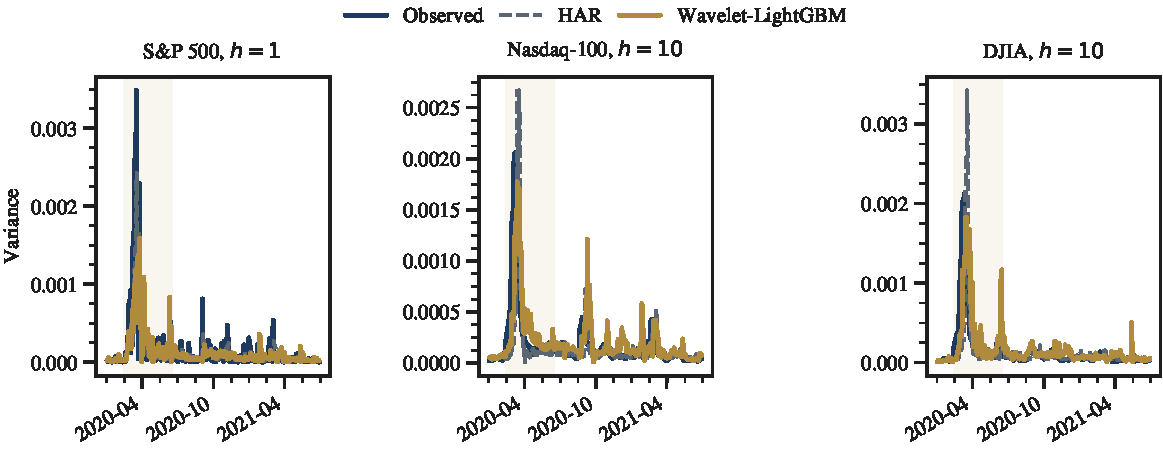
\includegraphics[width=0.94\textwidth]{figures/fig05_forecast_panels.pdf}
\caption{Representative out-of-sample forecast traces in the main and expanded-data specifications. The wavelet-enhanced model follows the build-up and decay of stress episodes more smoothly at \(h=5\) and \(h=10\), whereas isolated daily spikes still tend to favour the parsimonious HAR benchmark.}
\label{fig:forecast_panels_appendix}
\end{figure}

\begin{figure}[!t]
\centering
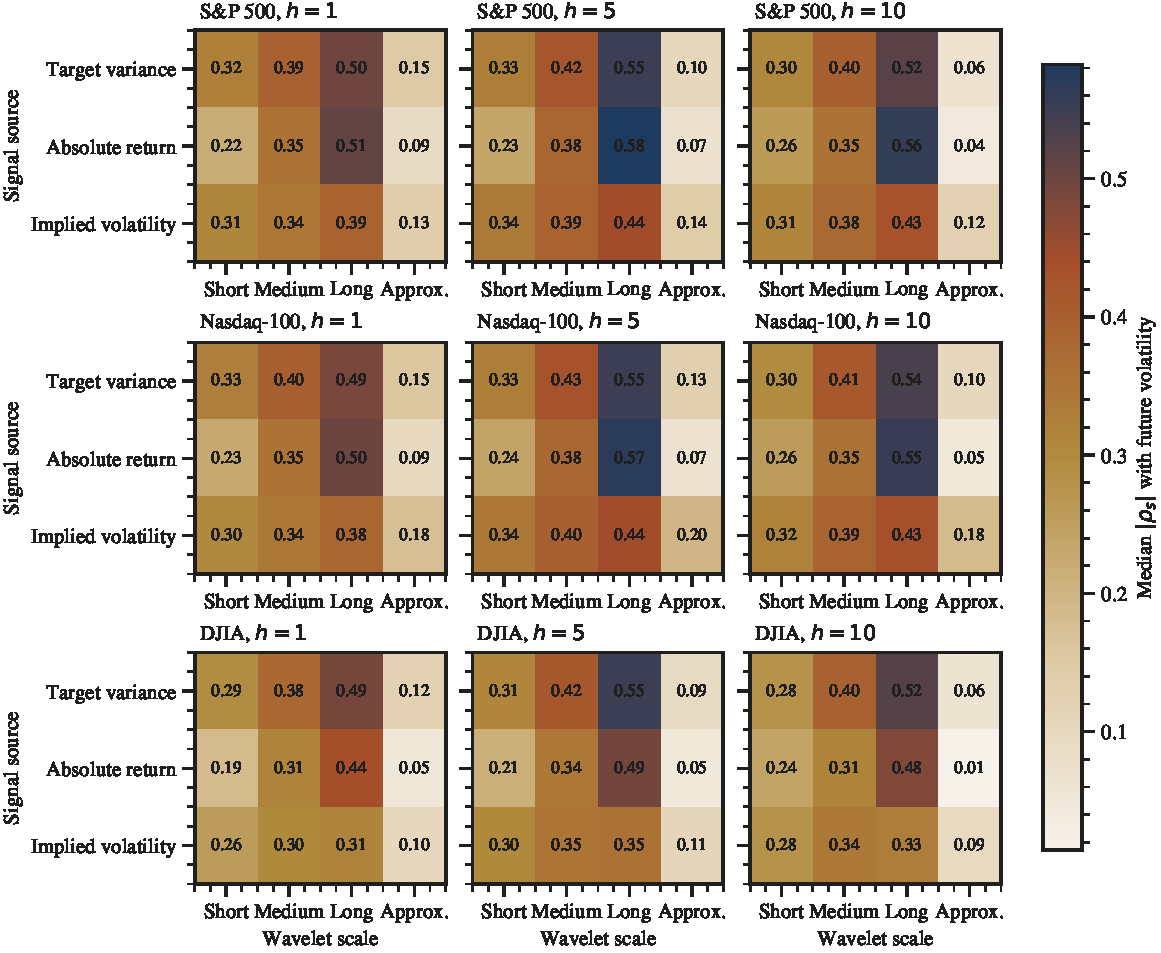
\includegraphics[width=0.94\textwidth]{figures/fig11_multiscale_signal_heatmap.pdf}
\caption{Multiscale signal map in the expanded public risk-data panel. Each cell reports the median absolute Spearman association between a wavelet feature group and future volatility.}
\label{fig:multiscale_signal_heatmap_appendix}
\end{figure}

\begin{figure}[!t]
\centering
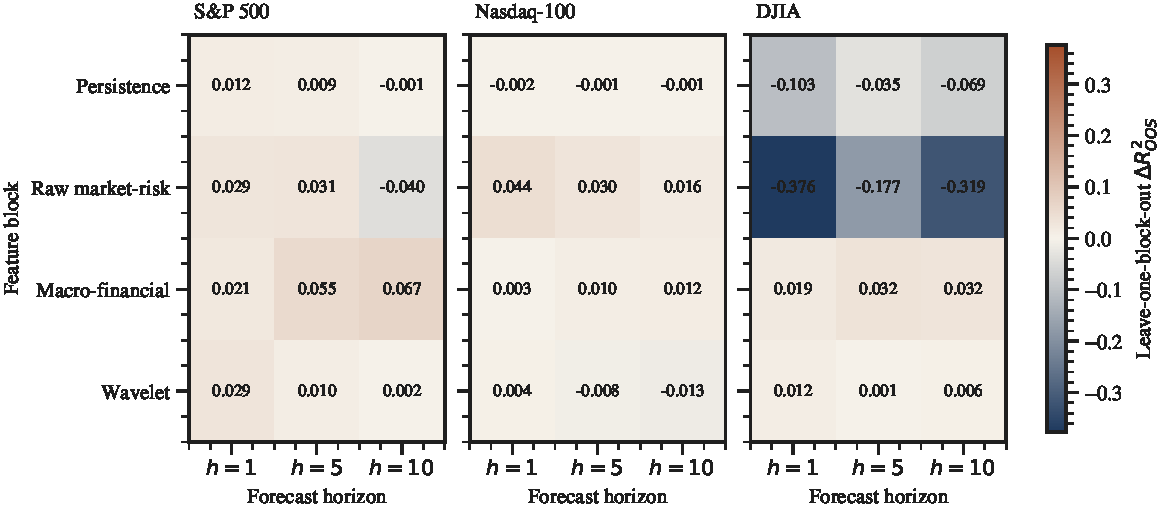
\includegraphics[width=0.94\textwidth]{figures/fig12_block_contribution_heatmap.pdf}
\caption{Surrogate leave-one-block-out contribution map in the expanded public risk-data panel. Each cell reports the change in out-of-sample \(R^2\) from removing one feature block from a fixed train/test surrogate regression on block embeddings.}
\label{fig:block_contribution_heatmap_appendix}
\end{figure}

\begin{figure}[!t]
\centering
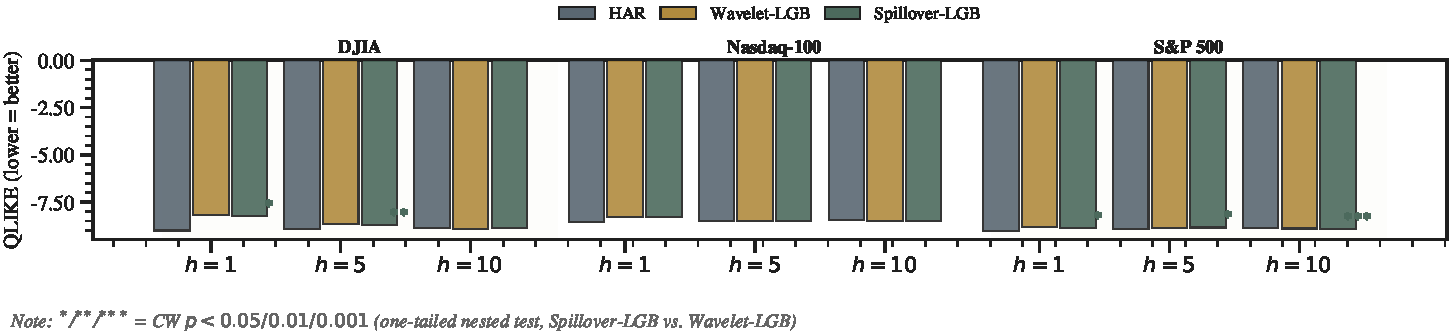
\includegraphics[width=0.94\textwidth]{figures/fig_spillover_qlike_bars.pdf}
\caption{QLIKE comparison across indices and forecast horizons for the three models in the spillover ablation. Asterisks above the Spillover-LGB bar indicate Clark--West significance at the corresponding cell.}
\label{fig:spillover_qlike_bars_appendix}
\end{figure}

\begin{figure}[!t]
\centering
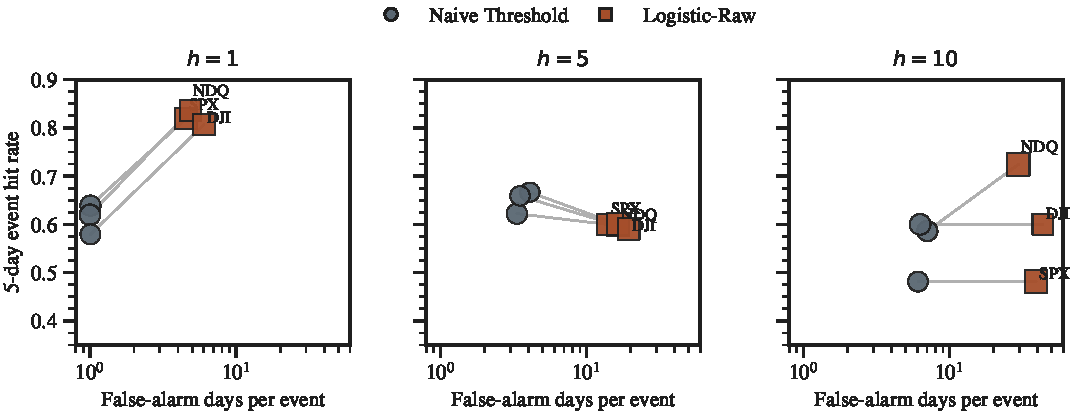
\includegraphics[width=0.96\textwidth]{figures/fig14_warning_event_frontier.pdf}
\caption{Event-based warning frontier at the index--horizon level. The horizontal axis reports false-alarm days per event on a log scale, the vertical axis reports the five-day event hit rate, and marker size scales with the mean lead time. Grey line segments connect the two warning rules within the same index--horizon cell.}
\label{fig:warning_event_frontier_appendix}
\end{figure}

\subsection{Additional Statistical Tables}

\begin{table}[!t]
\caption{Forecast comparison tests against HAR in the main specification.}
\label{tab:significance_tests}
\centering
\scriptsize
\setlength{\tabcolsep}{3.5pt}
\resizebox{\textwidth}{!}{%
\begin{tabular}{lllllll}
\toprule
Index & Horizon & Model & DM stat & DM p-value & CW stat & CW p-value \\
\midrule
DJIA & 1 & LightGBM & 3.572 & 0.0004 & 2.060 & 0.0197 \\
DJIA & 1 & Wavelet-LightGBM & 3.344 & 0.0008 & 2.440 & 0.0073 \\
DJIA & 5 & LightGBM & 1.925 & 0.0542 & 2.333 & 0.0098 \\
DJIA & 5 & Wavelet-LightGBM & 1.458 & 0.1448 & 2.503 & 0.0062 \\
DJIA & 10 & LightGBM & -0.228 & 0.8194 & 2.901 & 0.0019 \\
DJIA & 10 & Wavelet-LightGBM & -1.158 & 0.2467 & 2.983 & 0.0014 \\
Nasdaq-100 & 1 & LightGBM & 2.927 & 0.0034 & 2.935 & 0.0017 \\
Nasdaq-100 & 1 & Wavelet-LightGBM & 3.967 & 0.0001 & 3.542 & 0.0002 \\
Nasdaq-100 & 5 & LightGBM & -0.990 & 0.3224 & 4.516 & 0.0000 \\
Nasdaq-100 & 5 & Wavelet-LightGBM & -0.353 & 0.7239 & 4.927 & 0.0000 \\
Nasdaq-100 & 10 & LightGBM & -1.080 & 0.2801 & 4.682 & 0.0000 \\
Nasdaq-100 & 10 & Wavelet-LightGBM & -2.145 & 0.0320 & 4.821 & 0.0000 \\
S\&P 500 & 1 & LightGBM & 2.639 & 0.0083 & 2.641 & 0.0041 \\
S\&P 500 & 1 & Wavelet-LightGBM & 2.614 & 0.0090 & 2.669 & 0.0038 \\
S\&P 500 & 5 & LightGBM & 1.004 & 0.3155 & 2.489 & 0.0064 \\
S\&P 500 & 5 & Wavelet-LightGBM & 0.900 & 0.3683 & 2.678 & 0.0037 \\
S\&P 500 & 10 & LightGBM & -0.180 & 0.8572 & 2.784 & 0.0027 \\
S\&P 500 & 10 & Wavelet-LightGBM & 0.202 & 0.8398 & 2.736 & 0.0031 \\
\bottomrule
\end{tabular}
}
\end{table}


\begin{table}[!t]
\caption{Broad-market regime-conditioned spillover gains. Entries report $\Delta$QLIKE = Spillover-LGB minus Wavelet-LGB for DJIA and S\&P 500 pooled observations. Negative values indicate that cross-index spillover features improve accuracy.}
\label{tab:spillover_regime}
\centering
\small
\setlength{\tabcolsep}{5.0pt}
\renewcommand{\arraystretch}{1.10}
\begin{tabular}{lccc}
\toprule
Regime & $h=1$ & $h=5$ & $h=10$ \\
\midrule
Bottom 20\% VIX & -0.042 & 0.009 & -0.004 \\
COVID 2020--2021 & -0.377 & 0.122 & 0.011 \\
Expansion & -0.054 & -0.016 & \best{-0.006} \\
Post-2022 & -0.028 & -0.109 & -0.002 \\
Recession & \best{-0.674} & \best{-0.361} & 0.145 \\
Top 20\% VIX & -0.069 & -0.045 & -0.002 \\
\bottomrule
\end{tabular}
\end{table}


\subsection{Project Assets}

The core manuscript results are generated from three merged result packages: the main Rogers--Satchell specification, the expanded public risk-data specification, and the Parkinson specification. The manuscript figures and tables are produced from these merged packages through deterministic scripts stored in the project repository. This setup is intended to make the final article easy to audit, rerun, and extend.


\begin{adjustwidth}{-\extralength}{0cm}
\reftitle{References}
\bibliography{bib/references}
\end{adjustwidth}

\end{document}
